%  !TeX  root  =  user_guide.tex

\chapter{Integrazione con GRASS GIS}\label{sec:grass}\index{GRASS}

% when the revision of a section has been finalized,
% comment out the following line:
% \updatedisclaimer

Il plugin GRASS consente l'accesso ai dati e alle funzioni di GRASS
GIS~\cite{GRASSweb}, inclusa la visualizzazione di layer raster e vettoriali,
la digitalizzazione di layer vettoriali, la modifica degli attributi, la
creazione di nuovi vettori e l'analisi di dati GRASS 2D e 3D tramite più di
300 moduli GRASS.

Questa Sezione contiene un'introduzione sulle funzionalità del plugin
e qualche esempio sulla gestione e l'utilizzo di dati GRASS. Quando viene
abilitato il plugin GRASS, come descritto alla Sezione~\ref{sec:starting_grass},
le seguenti funzionalità sono disponibili nella barra degli strumenti GRASS:
 
\begin{itemize}[label=--]
\item \toolbtntwo{grass_open_mapset}{Apri mapset}
\item \toolbtntwo{grass_new_mapset}{Nuovo mapset}
\item \toolbtntwo{grass_close_mapset}{Chiudi mapset}
\item \toolbtntwo{grass_add_vector}{Aggiungi vettore GRASS}
\item \toolbtntwo{grass_add_raster}{Aggiungi raster GRASS}
\item \toolbtntwo{grass_new_vector_layer}{Crea nuovo vettore GRASS}
\item \toolbtntwo{grass_edit}{Modifica vettore GRASS}
\item \toolbtntwo{grass_tools}{Apri strumenti GRASS}
\item \toolbtntwo{grass_region}{Visualizza la regione di GRASS  attuale} 
\item \toolbtntwo{grass_region_edit}{Modifica la regione di GRASS attuale}
\end{itemize}

\subsection{Avviare il plugin GRASS}\label{sec:starting_grass}
\index{GRASS!avviare da QGIS}

Per usare le funzioni GRASS e/o visualizzare layer raster e vettoriali in
formato GRASS in QGIS, bisogna prima selezionare e caricare il plugin GRASS con il
gestore di plugin. 
Cliccare su \mainmenuopt{Plugins} \arrow \mainmenuopt{Gestione plugins...}, 
selezionare \dropmenuopt{GRASS} e cliccare su \button{OK}. 

Ora è possibile caricare layer raster e vettoriali da una \filename{LOCATION}
GRASS esistente (Sezione \ref{sec:load_grassdata}). È anche
possibile creare una nuova \filename{LOCATION} GRASS in QGIS (Sezione \ref{sec:create_loc}) 
e importarci dati raster e vettoriali (Si
veda la Sezione \ref{sec:import_loc_data}) per ulteriori analisi con gli
strumenti GRASS (Sezione \ref{subsec:grass_toolbox}).

\section{Caricare layer raster e vettoriali GRASS}\label{sec:load_grassdata}\index{GRASS!caricamento dati}

Con il plugin GRASS, possono essere caricati layer raster o vettoriali
usando il pulsante appropriato nella barra strumenti. Come esempio si
consideri il set di dati Alaska (Sezione \ref{label_sampledata}) che contiene una \filename{LOCATION} 
GRASS campione contenente tre layer vettoriali e una mappa di altitudine raster.

\begin{enumerate}
  \item Creare una nuova cartella \filename{grassdata}, nella quale scaricare
  il set di dati Alaska denominato \filename{qgis\_sample\_data.zip}
  dall'indirizzo web \url{http://download.osgeo.org/qgis/data/} e decomprimere
  il file nella cartella \filename{grassdata}.
  \item Avviare QGIS.
  \item Se non è già stato fatto in precedenti sessioni di QGIS, caricare il
  plugin GRASS cliccando su \mainmenuopt{Plugins} \arrow \mainmenuopt{Gestione
  Plugins...} e selezionare \dropmenuopt{GRASS}: apparirà la barra degli strumenti GRASS.
  \item Nella barra strumenti GRASS, cliccare sull'icona
  \toolbtntwo{grass_open_mapset}{Apri mapset} per aprire la finestra \filename{Scegli mapset GRASS}.
  \item Alla voce \filename{Gisdbase} inserire l'indirizzo completo o navigare
  fino alla cartella \filename{grassdata} appena creata.
  \item Dovrebbe ora essere possibile selezionare la \filename{LOCATION alaska} e il MAPSET \filename{demo}. 
  \item Cliccare su \button{OK}. Si noti che ora alcuni degli strumenti
  precedentemente disabilitati sono divenuti attivi.
  \item Cliccare su \toolbtntwo{grass_add_raster}{Aggiungi raster GRASS},
  scegliere la mappa denominata \filename{gtopo30} e cliccare su \button{OK}.
  Verrà visualizzato il layer delle quote del terreno.
  \item Cliccare su \toolbtntwo{grass_add_vector}{Aggiungi vettore GRASS},
  selezionare la mappa denominata \filename{alaska} e cliccare su \button{OK}.
  Il confine dell'Alaska verrà sovrapposto alla mappa gtopo30 map. Ora è
  possibile adattare le proprietà del layer come descritto al capitolo
  \ref{sec:vectorprops}, ovvero cambiare la trasparenza, il colore di
  riempimento e del contorno dell'elemento.
  \item Caricare anche gli altri due layer vettoriali denominati
  \filename{rivers} e \filename{airports} e modificarne le proprietà.
\end{enumerate}

È molto semplice caricare dati raster e vettoriali in
formato GRASS in QGIS. Si veda la sezione seguente per sapere come modificare
dati GRASS e creare nuove \filename{LOCATION}. Ulteriori \filename{LOCATION}
campione di GRASS sono disponibili sul sito web di GRASS all'indirizzo
\url{http://grass.osgeo.org/download/data.php}.

\begin{Tip}\caption{\textsc{Caricare dati GRASS}}
Se si presentano problemi nel caricare dati o QGIS termina
inaspettatamente, assicurarsi di aver caricato il plugin GRASS correttamente
come descritto alla Sezione \ref{sec:starting_grass}.
\end{Tip} 

\section{LOCATION e MAPSET in GRASS}\label{sec:about_loc}

GRASS organizza i propri dati in cartelle alle quali si fa riferimento con la
denominazione GISDBASE. Queste cartelle, spesso chiamate \filename{grassdata},
devono essere create prima di iniziare a lavorare con il plugin GRASS in QGIS.
In queste directory, i dati GRASS sono organizzati per progetti inseriti in
sottocartelle chiamate \filename{LOCATION}. 
Ogni \filename{LOCATION} è definita da un sistema di coordinate, da una 
proiezione e dall'estensione geografica. La \filename{LOCATION} può avere a
sua volta molte sottocartelle denominate \filename{MAPSET} usate per suddividere il
progetto in diversi argomenti, sottoregioni o spazi di lavoro per i diversi
membri del team che vi sta lavorando (Neteler \& Mitasova 2008
\cite{neteler_mitasova08}). Per analizzare layer raster e vettoriali con i
moduli GRASS, bisogna importarli in una \filename{LOCATION} GRASS.
\footnote{Questo non è del tutto vero - con i moduli GRASS \filename{r.external}
e \filename{v.external} è possibile creare collegamenti in sola lettura ai
dati GDAL/OGR supportati senza che sia necessario effettuare l'importazione.
Tuttavia siccome questa non è la modalità predefinita per i principianti, 
questa funzione non verrà descritta.}

\begin{figure}[ht]
\centering

\includegraphics[clip=true]{grass_location}
\caption{Organizzazzione dei dati GRASS nella LOCATION campione alaska
(adattato da Neteler \& Mitasova 2008 \cite{neteler_mitasova08})}\label{fig:grass_location}
\end{figure}

\subsection{Creare una nuova LOCATION GRASS}\label{sec:create_loc}

Per questo e per tutti i successivi esempi riguardanti GRASS GIS verrà usata la \filename{LOCATION
alaska} campione, nel sistema di riferimento Albers Equal Area, unità di misura in metri e 
creata dal set di dati campione di QGIS. Sarà utile scaricare
ed installare il set di dati sul proprio computer (\ref{label_sampledata}).

\begin{figure}[ht]
\centering
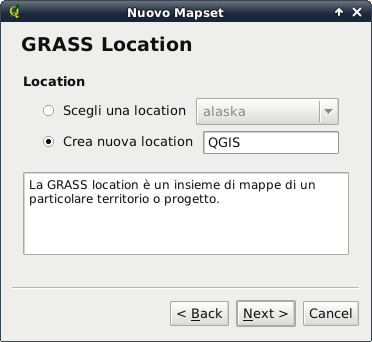
\includegraphics[clip=true, width=8cm]{create_grass_location}
\caption{Creazione di una nuova LOCATION \grass o di un nuovo MAPSET in \qg \nixcaption}
\label{fig:create_grass_location}
\end{figure}

\begin{enumerate}
  \item Avviare QGIS e assicurarsi che il plugin GRASS sia caricato
  \item Visualizzare lo shapefile \filename{alaska.shp} (Sezione
  \ref{sec:load_shapefile}) dal set di dati alaska~(\ref{label_sampledata}).
  \item Nella barra strumenti GRASS, cliccare sull'icona
  \toolbtntwo{grass_new_mapset}{Nuovo mapset} per avviare la procedura guidata.
  \item Selezionare la cartella contenente il database GRASS (GISDBASE)
  denominata \filename{grassdata} o crearne una nuova in cui ospitare la nuova
  \filename{LOCATION} usando il gestore di file installato sul proprio
  computer. Cliccare su \button{Next}. 
  \item Per creare un nuovo \filename{MAPSET} in una \filename{LOCATION}
  esistente (Sezione~\ref{sec:add_mapset}) o per creare una nuova
  \filename{LOCATION}, selezionare l'opzione \radiobuttonon{Crea nuova
  location} (Figura \ref{fig:create_grass_location}).
  \item Inserire il nome della \filename{LOCATION} - nell'esempio abbiamo
  usato alaska, e cliccare su \button{Next} 
  \item Definire la proiezione cliccando sull'opzione
  \radiobuttonon{Proiezione} per abilitare l'elenco delle proiezioni 
  \item Scegliere la proiezione Albers Equal Area Alaska (feet). Siccome ne
  conosciamo l'identificativo EPSG 2964, inserirlo nella casella di
  ricerca. (Nota: se si vuole ripetere il processo per un'altra
  \filename{LOCATION} e non si è memorizzato l'identificativo EPSG della
  proiezione, cliccare sull'icona \toolbtntwo{mIconProjectionEnabled}{Stato SR}
  a destra nella barra di stato (Sezione \ref{label_projstart})).
  \item Cliccare su \button{Trova} per selezionare la proiezione
  \item Cliccare su \button{Next} 
  \item Per definire l'estensione della regione predefinita, bisogna inserire i
  limiti della \filename{LOCATION} verso nord, sud, est e ovest. Nel nostro
  esempio cliccare semplicemente sul pulsante \button{Imposta estensione
  attuale di QGIS}, per applicare l'estensione del layer caricato
  \filename{alaska.shp} come estensione predefinita della regione GRASS.
  \item Cliccare su \button{Next} 
  \item Abbiamo anche bisogno di definire un \filename{MAPSET} interno alla
  location \filename{LOCATION}. Il nome è a scelta, nell'esempio abbiamo
  usato demo.
  \footnote{Quando si crea una nuova \filename{LOCATION}, GRASS crea
  automaticamente un \filename{MAPSET} speciale chiamato \filename{PERMANENT}
  designato a contenere i dati di base del progetto, l'estensione spaziale predefinita 
  e la definizione del sistema di coordinate (Neteler \& Mitasova 2008 
  \cite{neteler_mitasova08}).}
  \item Controllare il riassunto per assicurarsi che le impostazioni siano
  corrette e cliccare su \button{Finish} 
  \item La nuova \filename{LOCATION alaska} e i \filename{MAPSETs demo}
  e \filename{PERMANENT} vengono creati. Il set di lavoro impostato per il
  lavoro corrente è il \filename{MAPSET demo}.
  \item Si noti che alcuni strumenti della barra di GRASS precedentemente
  disabilitati sono ora attivi.
\end{enumerate}

Per quanto possa sembrare lunga, questa procedura costituisce un modo
veloce per creare una \filename{LOCATION}. La \filename{LOCATION alaska} è ora
pronta per l'importazione dei dati (Sezione \ref{sec:import_loc_data}).
È possibile usare dati raster e vettoriali della
\filename{LOCATION alaska} inclusa del set di dati 'alaska' di QGIS (\ref{label_sampledata})
e procedere alla Sezione \ref{label_vectmodel}.

\subsection{Aggiungere un nuovo MAPSET}\label{sec:add_mapset}

Ogni utente ha accesso in scrittura solo ai \filename{MAPSET} GRASS che ha
creato. Ciò implica che oltre ad accedere ai propri \filename{MAPSET},
l'utente può anche leggere i dati contenuti nei \filename{MAPSET} creati da
altri, ma può modificare o rimuovere solo i dati nei suoi \filename{MAPSET}.
Tutti i \filename{MAPSET} includono un file denominato \filename{WIND} nel
quale sono memorizzate le coordinate dei limiti della regione e la risoluzione 
spaziale impostata per i raster (Neteler \& Mitasova 2008
\cite{neteler_mitasova08} (Sezione \ref{sec:grass_region})). 
Per creare un nuovo \filename{MAPSET}:

\begin{enumerate}
  \item Avviare QGIS e assicurarsi che il plugin GRASS sia abilitato
  \item Nella barra degli strumenti GRASS, cliccare sull'icona
  \toolbtntwo{grass_open_mapset}{Apri mapset} per avviare la procedura guidata
  di creazione del \filename{MAPSET}.
  \item Selezionare la cartella GRASS (GISDBASE) \filename{grassdata} con il
  nome \filename{LOCATION alaska}, nel quale si vuole aggiungere un ulteriore
  \filename{MAPSET}, che chiameremo test.
  \item Cliccare su \button{Next}. 
  \item Con questa procedura possiamo creare un nuovo \filename{MAPSET}
  all'interno di una \filename{LOCATION} esistente e creare anche una nuova
  \filename{LOCATION} contemporaneamente. Cliccare sull'opzione
  \radiobuttonon{Selezionare location} (Figura \ref{fig:create_grass_location}) e cliccare su \button{Next}.
  \item Inserire il nome \filename{test} per il nuovo \filename{MAPSET}. Più
  sotto nella finestra è visibile una lista di \filename{MAPSETs} esistenti e
  i relativi proprietari.
  \item Cliccare su \button{Next}, controllare il riassunto per
  assicurarsi che le impostazioni siano corrette e cliccare su \button{Finish}.
\end{enumerate}

\subsection{Importare dati nelle LOCATION GRASS}\label{sec:import_loc_data}

Questa Sezione fornisce un esempio su come importare dati raster e vettoriali
nella \filename{LOCATION} GRASS \filename{alaska} fornita dal set di dati QGIS
alaska. Verrà usata la mappa raster dell'uso del suolo \filename{landcover.img} e
il file vettoriale GML \filename{lakes.gml}.

\begin{enumerate}
  \item Avviare QGIS e assicurarsi che il plugin GRASS sia caricato.
  \item Nella barra degli strumenti GRASS, cliccare sull'icona
  \toolbtntwo{grass_open_mapset}{Apri MAPSET} per aprire la finestra di
  selezione \filename{MAPSET}.
  \item Selezionare come GRASS database la cartella \filename{grassdata} nel
  set di dati QGIS alaska, come \filename{LOCATION alaska}, come
  \filename{MAPSET} \filename{demo} e cliccare su \button{OK}.
  \item Cliccare ora sullo strumento \toolbtntwo{grass_tools}{Apri strumenti
  GRASS}. Apparirà la finestra degli strumenti di GRASS (Sezione \ref{subsec:grass_toolbox}).
  \item Per importare la mappa raster \filename{landcover.img}, cliccare sul
  modulo \filename{r.in.gdal} nella scheda \tab{Albero moduli}. Questo
  modulo GRASS consente l'importazione di file supportati da GDAL in una
  \filename{LOCATION} GRASS. Apparirà la finestra di dialogo del modulo
  \filename{r.in.gdal}.
  \item Navigare alla cartella \filename{raster} nel set
  di dati QGIS alaska e selezionare il file \filename{landcover.img}.
  \item Come nome del raster in uscita inserire \filename{landcover\_grass} e
  cliccare su \button{Esegui}. Nella scheda \tab{Output} è possibile
  verificare l'avanzamento del comando GRASS \filename{r.in.gdal -o
  input=/path/to/landcover.img output=landcover\_grass}.
  \item Quando compare la dicitura \textbf{Operazione conclusa con successo}
  cliccare sul pulsante \button{Visualizza output}. Il layer raster
  \filename{landcover\_grass} è ora importato in GRASS e verrà visualizzato
  nella vista mappa di QGIS.
  \item Per importare il vettore \filename{lakes.gml},
  usare il modulo \filename{v.in.ogr} nella scheda \tab{Albero moduli}.
  Questo modulo GRASS consente di importare i formati vettoriali supportati da
  OGR in una \filename{LOCATION} GRASS. Apparirà la finestra di dialogo \filename{v.in.ogr}.
  \item Navigare alla cartella \filename{gml} nel set di dati
  QGIS alaska e selezionare il file \filename{lakes.gml} come file OGR.
  \item Come nome del vettore in uscita inserire
  \filename{lakes\_grass} e cliccare su \button{Esegui}. In questo esempio è
  possibile trascurare le altre opzioni. Nella scheda \tab{Output} è
  possibile verificare l'avanzamento del comando GRASS \filename{v.in.ogr -o
  dsn=/path/to/lakes.shp output=lakes\_grass}.
  \item Quando compare la dicitura \textbf{Operazione conclusa con successo}
  cliccare su \button{Visualizza output}. Il layer vettoriale
  \filename{lakes\_grass} è ora importato in grass e verrà visualizzato nella
  vista mappa di QGIS. 
\end{enumerate}

\section{Il modello dati vettoriale di GRASS}\label{label_vectmodel}\index{GRASS!modello dati vettoriale}

È importante comprendere il modello dati vettoriale di GRASS, per gestire nella 
maniera ottimale le attività di digitalizzazione.\index{GRASS!digitalizzazione} 
In generale, GRASS usa un modello dati vettoriale topologico.\index{GRASS!topologia} 
Questo significa che le aree non sono rappresentate con poligoni chiusi singoli, 
ma da uno o più contorni (boundary). Un  contorno tra due aree adiacenti è digitalizzato una
sola volta e condiviso da entrambe le aree. Perché un'area sia topologicamente corretta, 
i contorni devono essere connessi senza soluzione di continuità. Un'area è identificata 
(ed etichettata) dal suo \textbf{centroide}.

Oltre a contorni e centroidi, una mappa vettoriale può contenere anche punti e
linee. Tutti questi elementi possono essere compresenti in un singolo layer
vettoriale e saranno rappresentati con 'livelli' differenti in una mappa vettoriale GRASS. 
Quindi in GRASS con 'layer' non s'intende una mappa raster o vettoriale bensì un livello 
all'interno di un dato vettoriale.
Questa è una distinzione molto importante da tenere presente.
\footnote{Sebbene sia possibile mescolare elementi geometrici di diverso tipo
(punti, linee, contorni e centroidi), ciò è abbastanza insolito e perfino in
GRASS viene usato solo in casi speciali come ad es. quando si esegue l'analisi
di una rete vettoriale. Di solito è preferibile che elementi geometrici
diversi vengano digitalizzati su "file" distinti.}

È possibile salvare più 'livelli' in un set di dati vettoriale. Per esempio
campi, foreste e laghi possono essere salvati in un vettore. Foreste e
laghi adiacenti possono condividere lo stesso contorno, ma avranno tabelle degli
attributi distinte. È anche possibile assegnare attributi ai contorni. Ad
esempio se il contorno tra un lago ed una foresta è una strada, questa può avere una
diversa tabella degli attributi.
 
Il livello di un elemento è definito "layer" in GRASS. "Layer" è il numero che 
indica se c'è più di un gruppo geometrico nel set di dati vettoriale, ad es. se 
la geometria è foresta o lago. Attualmente tale indice può essere
solo un numero, in versioni di GRASS successive saranno supportati anche stringhe di testo.

Gli attributi degli elementi geometrici possono essere memorizzati nella
\filename{LOCATION} GRASS in formato DBase o SQLITE3 o in database esterni
come PostgreSQL, MySQL, Oracle, ecc.\index{GRASS!archiviazione attributi}

Gli attributi contenuti nelle tabelle del database sono collegati alla 
geometria per il tramite di un valore 'category'.\index{GRASS!collegamento attributi}
'Category' (key, ID) è un valore intero collegato alle primitive geometriche
ed è usato come collegamento ad una colonna chiave nella tabella del database.

\begin{Tip}\caption{\textsc{Conoscere il modello dati vettoriale di GRASS}}
Il miglior modo per capire il modello dati vettoriale di GRASS e le sue
capacità è quello di scaricare una delle molte guide (tutorial) di GRASS nelle 
quali tale modello è descritto più approfonditamente. Si veda
\url{http://grass.osgeo.org/gdp/manuals.php} per informazioni, libri e
guide in diverse lingue.
\end{Tip} 

\section{Creare un nuovo layer vettoriale GRASS}\label{sec:creating_new_grass_vectors}\index{GRASS!creare nuovo layer vettoriale}

Per creare un nuovo layer vettoriale GRASS tramite il plugin GRASS cliccare
sullo strumento \toolbtntwo{grass_new_vector_layer}{Crea un nuovo vettore GRASS}. 
Inserire un nome nella casella di testo e iniziare la digitalizzazione di
punti, linee o poligoni, seguendo la procedura descritta alla Sezione
\ref{grass_digitising}. 

In GRASS è possibile gestire ogni tipo di geometria (punti, linee
ed aree) in un singolo layer, in quanto viene impiegato un modello dati
vettoriale topologico; di conseguenza non è necessario definire a priori il tipo di
geometria che si intende utilizzare per un nuovo vettore. 
In questo il modello dati di GRASS si differenzia ad esempio dal formato shapefile, 
che usa un modello vettoriale denominato Simple Feature (Sezione \ref{sec:create shape}).

\begin{Tip}\caption{\textsc{Creare una tabella attributi per un nuovo layer vettoriale GRASS}}
Se si desidera assegnare attributi alla geometria digitalizzata, accertarsi di
definire lo schema della tabella prima di iniziare a digitalizzare (Figura \ref{fig:grass_digitizing_table}).
\end{Tip} 

\section{Digitalizzare e modificare layer vettoriali GRASS}\index{GRASS!strumenti di digitalizzazione}\label{grass_digitising}

Gli strumenti di digitalizzazione per i layer vettoriali GRASS sono
accessibili con l'icona \toolbtntwo{grass_edit}{Modifica vettore GRASS}
nella barra degli strumenti GRASS. Assicurarsi di caricare un vettoriale GRASS e che esso
sia selezionato nella legenda prima di attivare lo strumento di
digitalizzazione. La Figura \ref{fig:grass_digitizing_category} mostra la
finestra di dialogo degli strumenti di digitalizzazione GRASS che viene mostrata quando
si clicca sullo strumento di modifica. Gli strumenti e le impostazioni di
questa barra saranno discussi nelle sezioni seguenti.

\begin{Tip}\caption{\textsc{Digitalizzare poligoni in GRASS}}
Per creare poligoni in GRASS, bisogna iniziare con il digitalizzarne i
contorni, impostando preliminarmente il modo \usertext{Nessuna categoria}.
Una volta chiuso il poligono, aggiungere un centroide (punto
dell'etichetta) all'interno del contorno chiuso impostando preliminarmente
la modalità \usertext{Prossimo non in uso}.
Questa procedura è necessaria in quanto il modello di dati vettoriale
topologico collega le informazioni sull'attributo del poligono sempre al
centroide e non al contorno.
\end{Tip} 

\minisec{Barra degli strumenti di digitalizzazione}\label{label_grasstoolbar}

Nella Figura \ref{fig:grass_digitizing_toolbar} sono mostrate le icone della
barra degli strumenti per la digitalizzazione del plugin GRASS. La
Tabella \ref{tab:grass_tools} mostra le funzioni disponibili.

\begin{figure}[h]
   \centering
   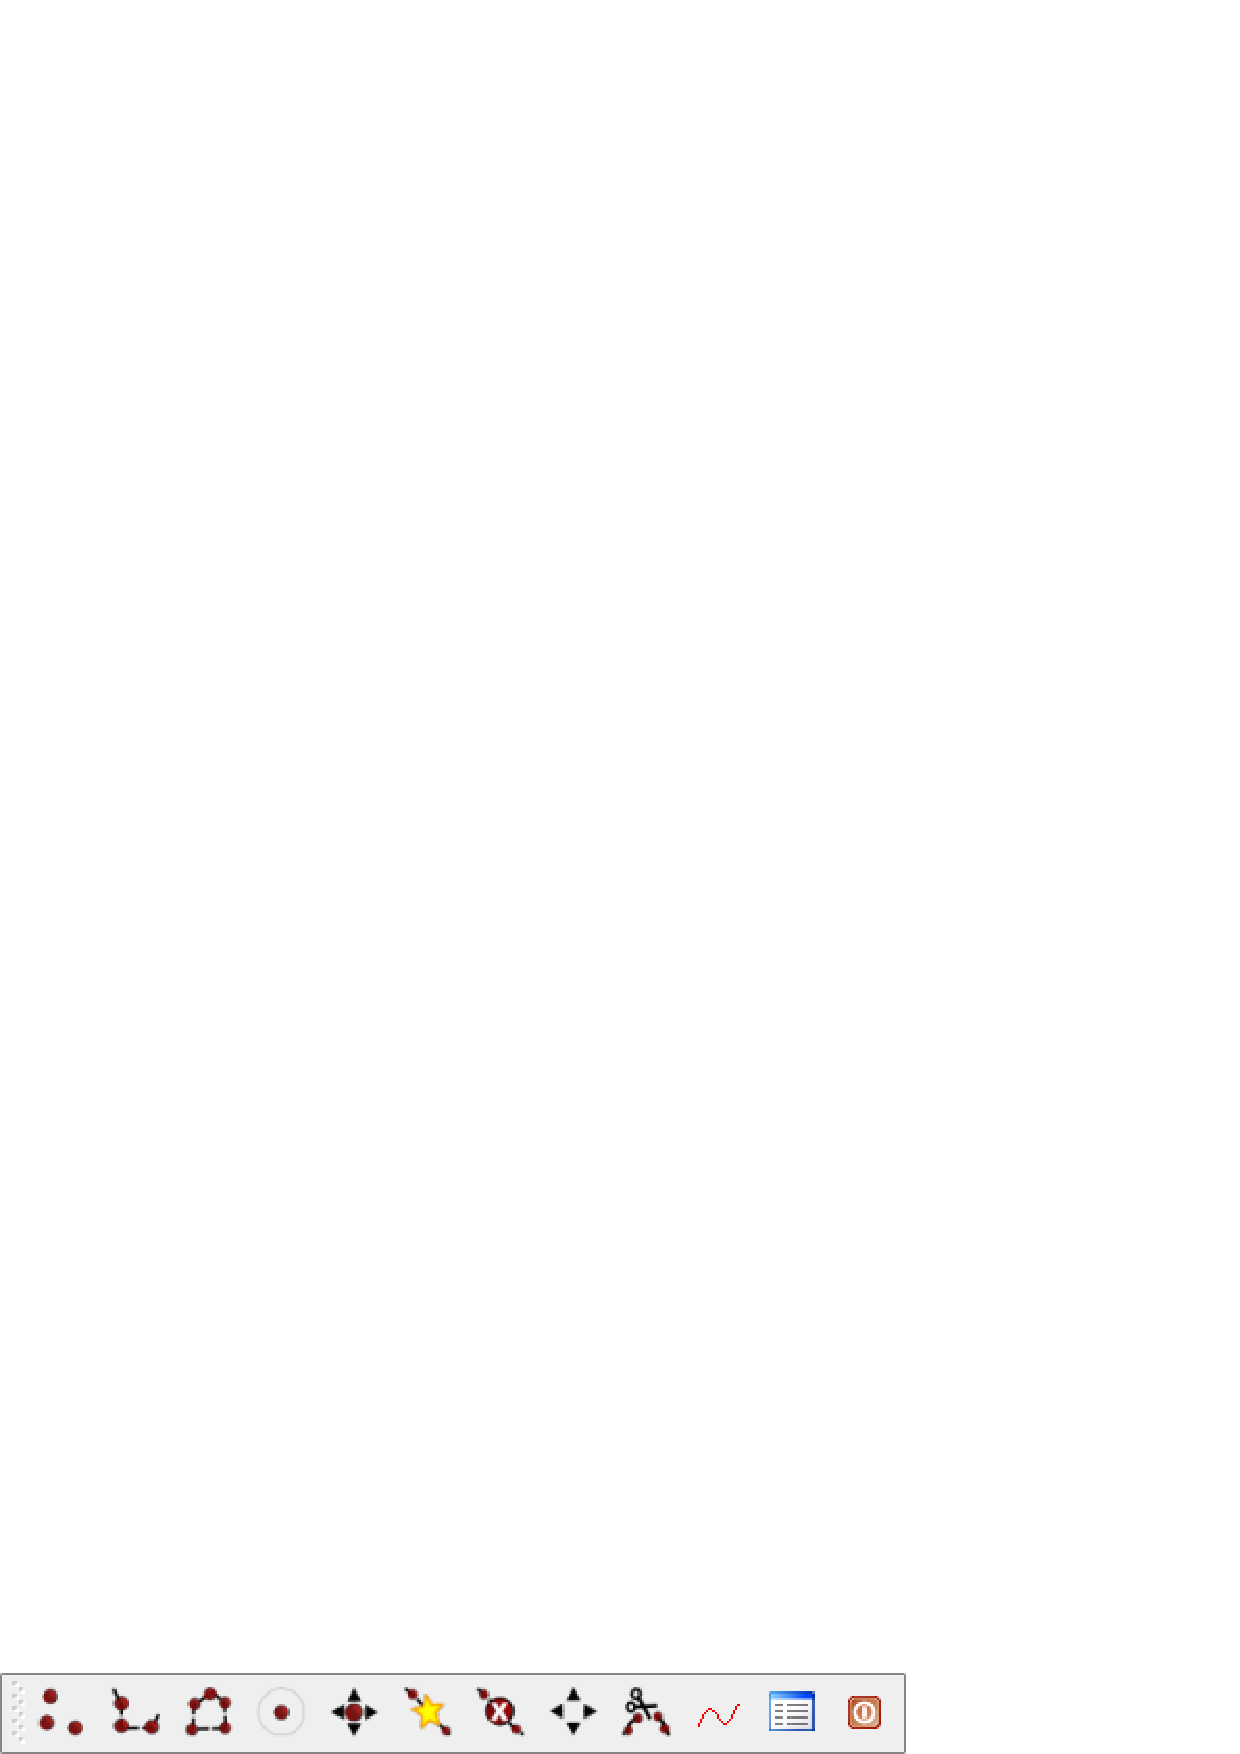
\includegraphics[clip=true,width=12cm]{grass_digitizing_toolbar}
   \caption{Barra degli strumenti di digitalizzazione GRASS \nixcaption}\label{fig:grass_digitizing_toolbar}
\end{figure}

\begin{table}[h]\index{GRASS!digitalizzazione strumenti}
\centering
\caption{Strumenti per la digitalizzazione in GRASS}\label{tab:grass_tools}\medskip
 \begin{tabular}{|l|l|p{5in}|}
 \hline \textbf{Icona} & \textbf{Strumento} & \textbf{Azione} \\
\hline 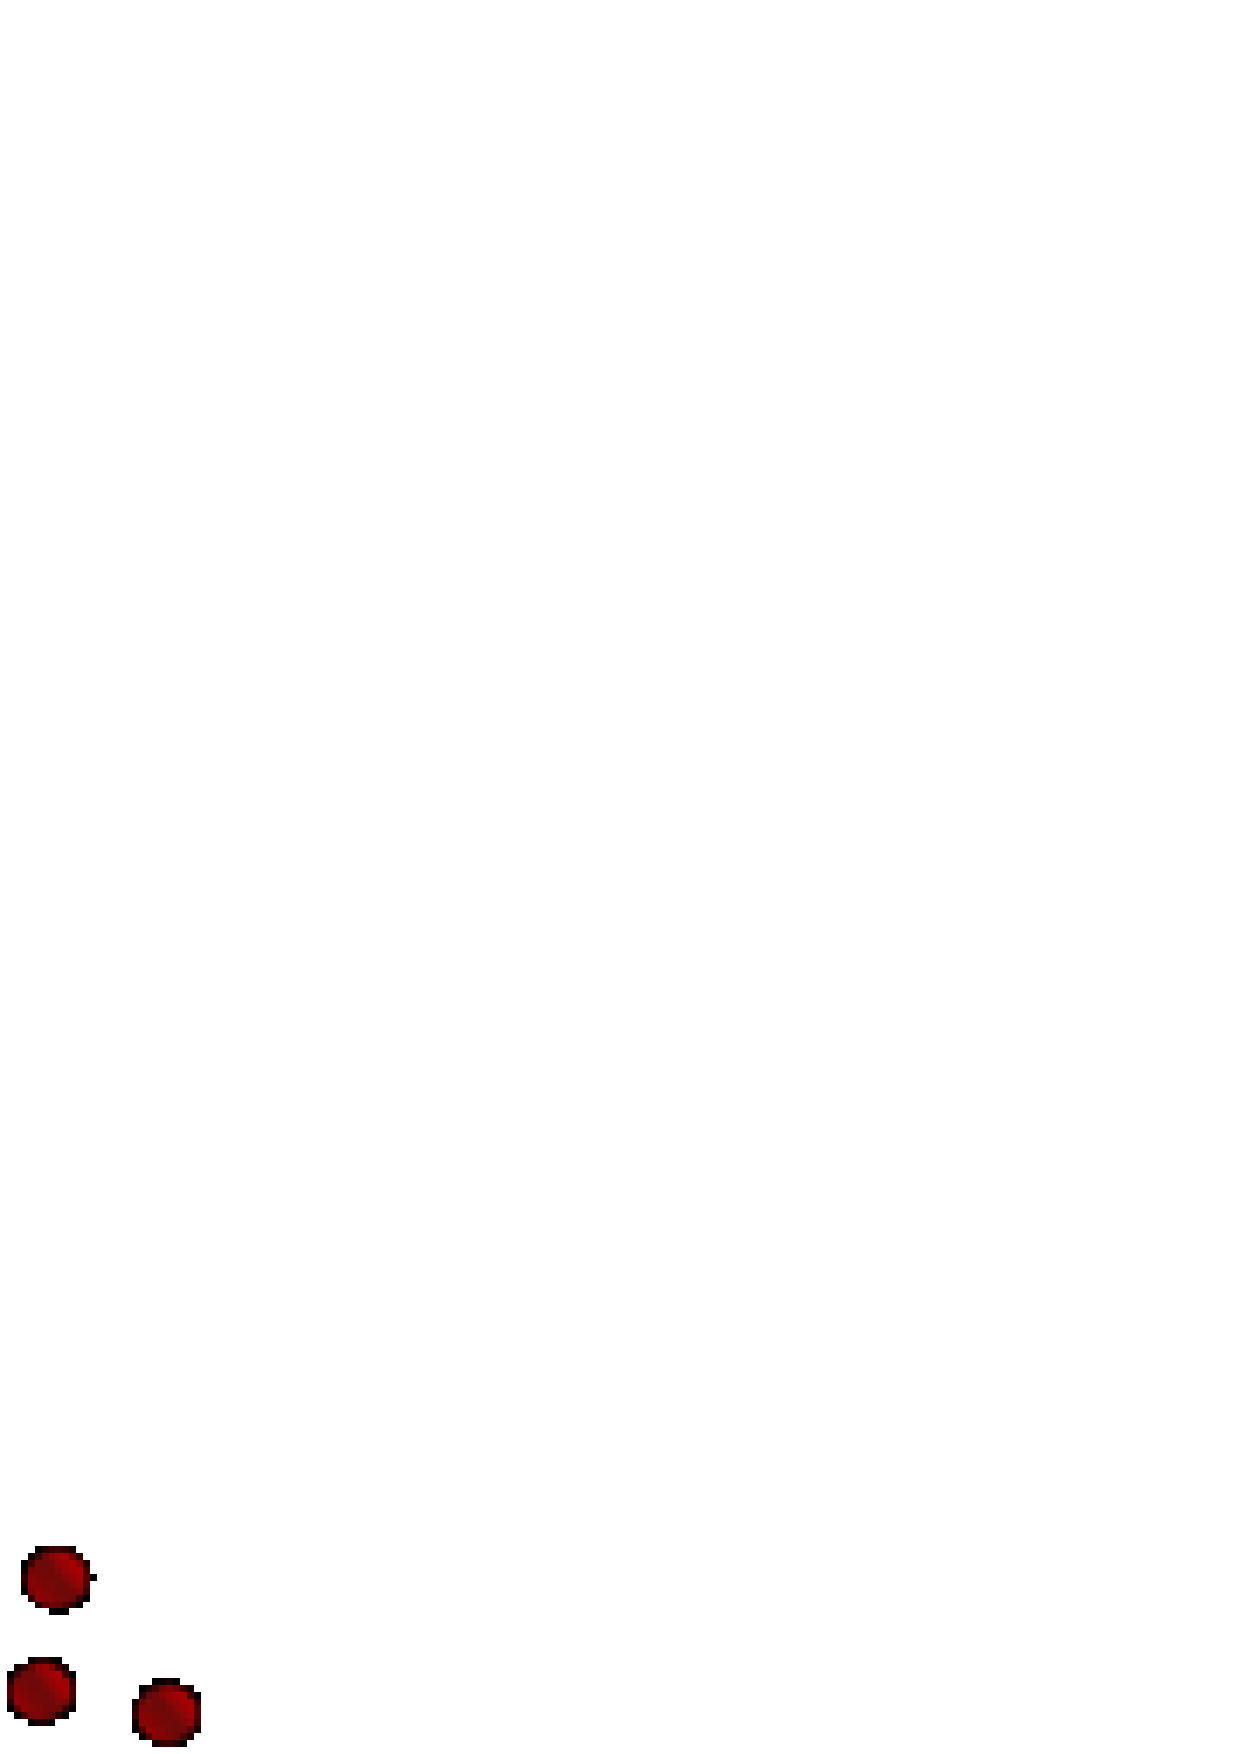
\includegraphics[width=0.7cm]{grass_new_point} & Nuovo punto &
Digitalizza un nuovo punto \\
\hline 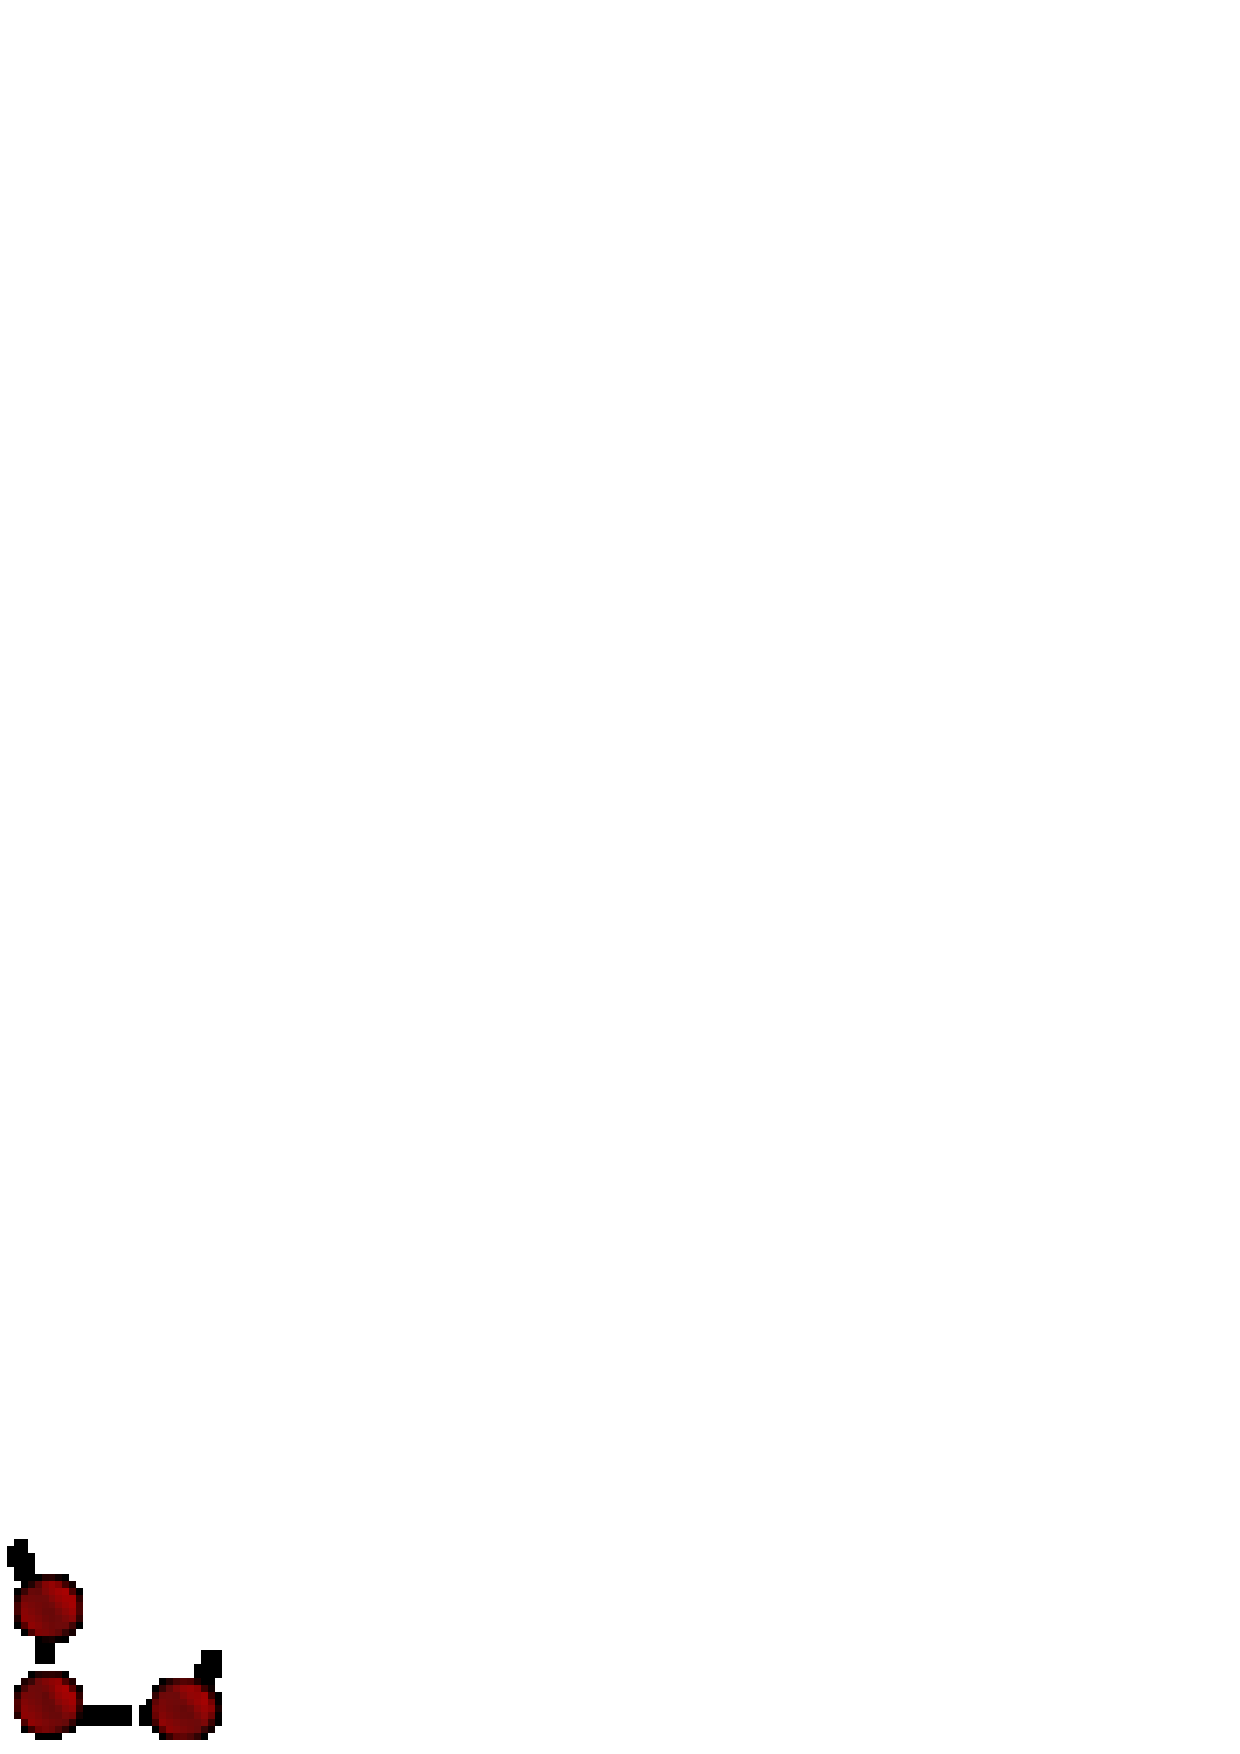
\includegraphics[width=0.7cm]{grass_new_line} & Nuova linea &
Digitalizza una nuova linea (annullare selezionando un altro strumento) \\
\hline 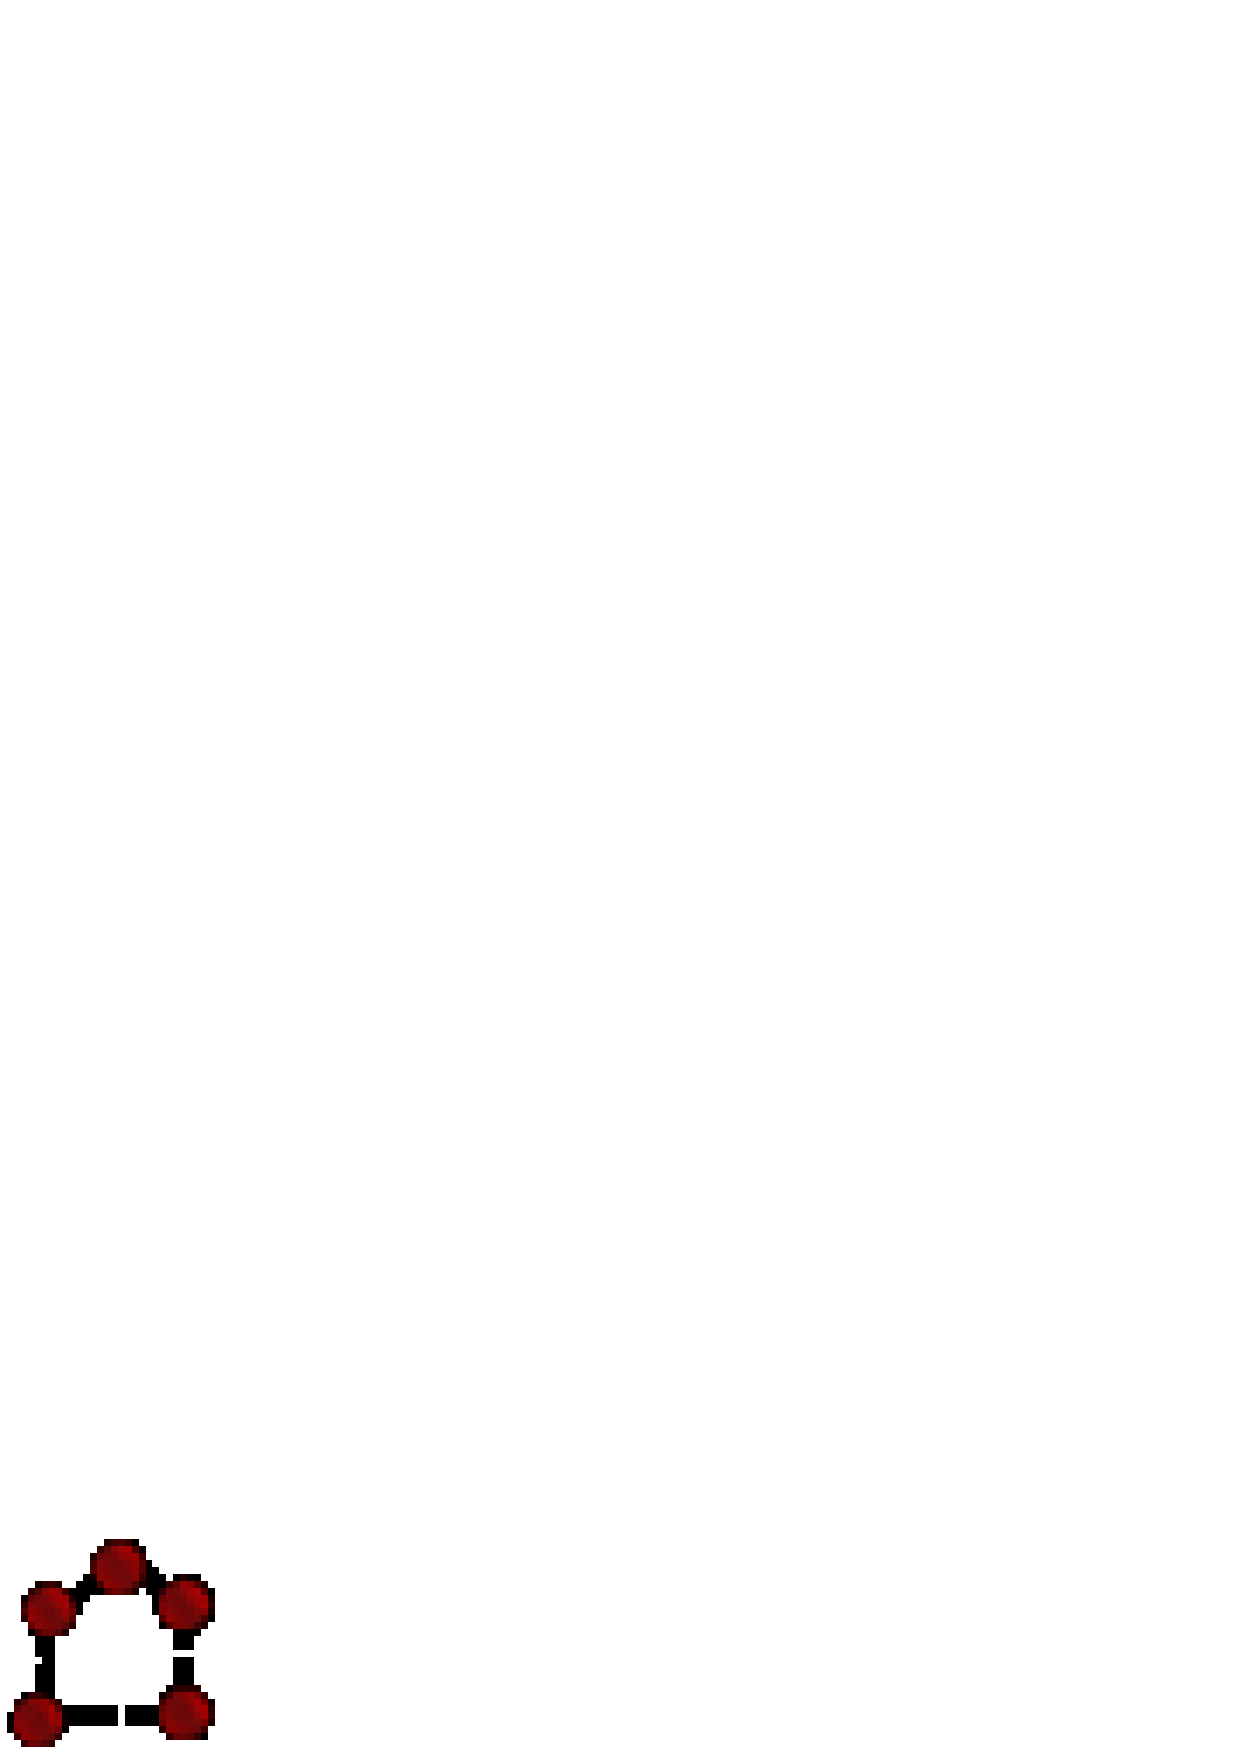
\includegraphics[width=0.7cm]{grass_new_boundary} & Nuovo contorno &
Digitizalizza nuovo contorno (annullare selezionando un altro strumento)\\
\hline 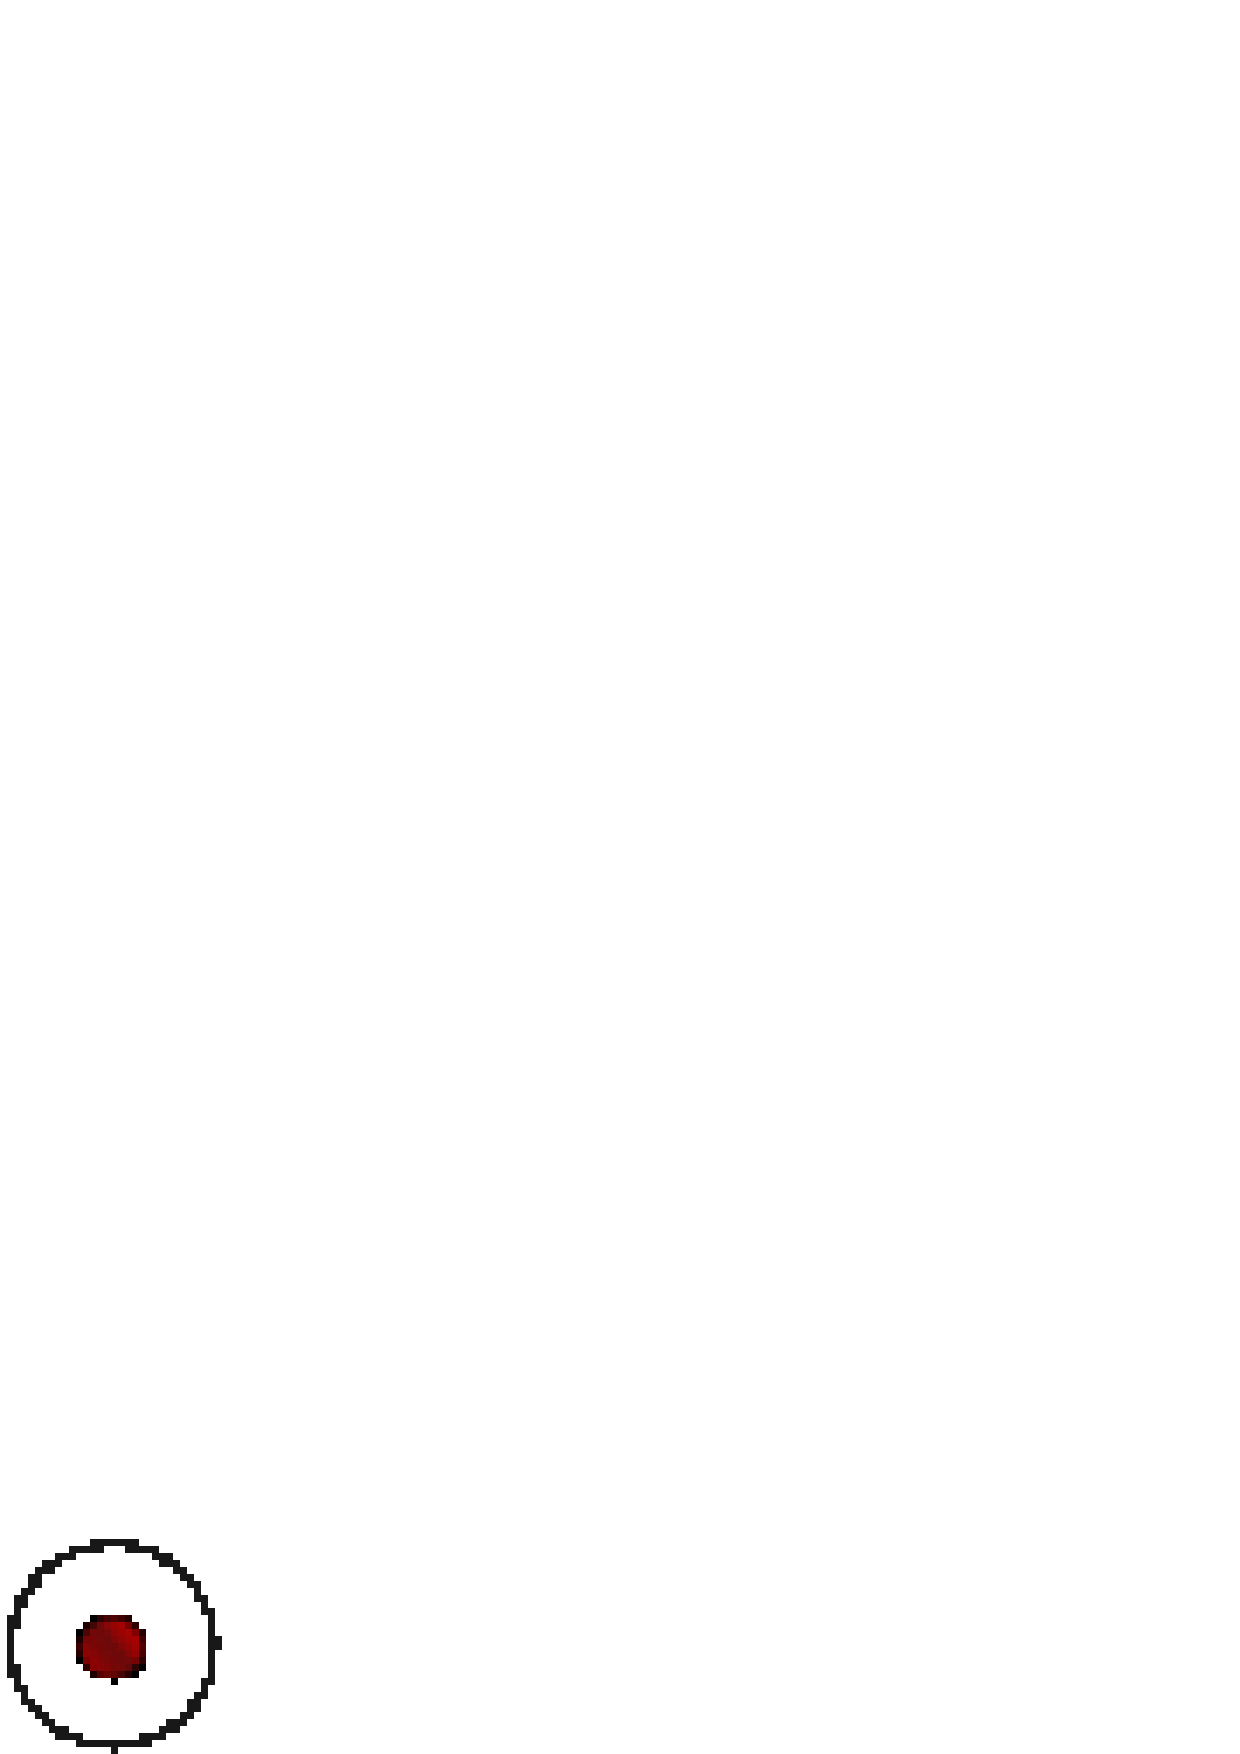
\includegraphics[width=0.7cm]{grass_new_centroid} & Nuovo centroide &
Digitalizza un nuovo centroide (imposta l'etichetta per un'area esistente)\\
\hline 
\includegraphics[width=0.7cm]{grass_move_vertex} & Sposta vertice &
Sposta un vertice di una linea o contorno esistente in una nuova posizione\\
\hline 
\includegraphics[width=0.7cm]{grass_add_vertex} & Aggiungi vertice &
Aggiunge un vertice ad una linea o contorno esistente\\
\hline 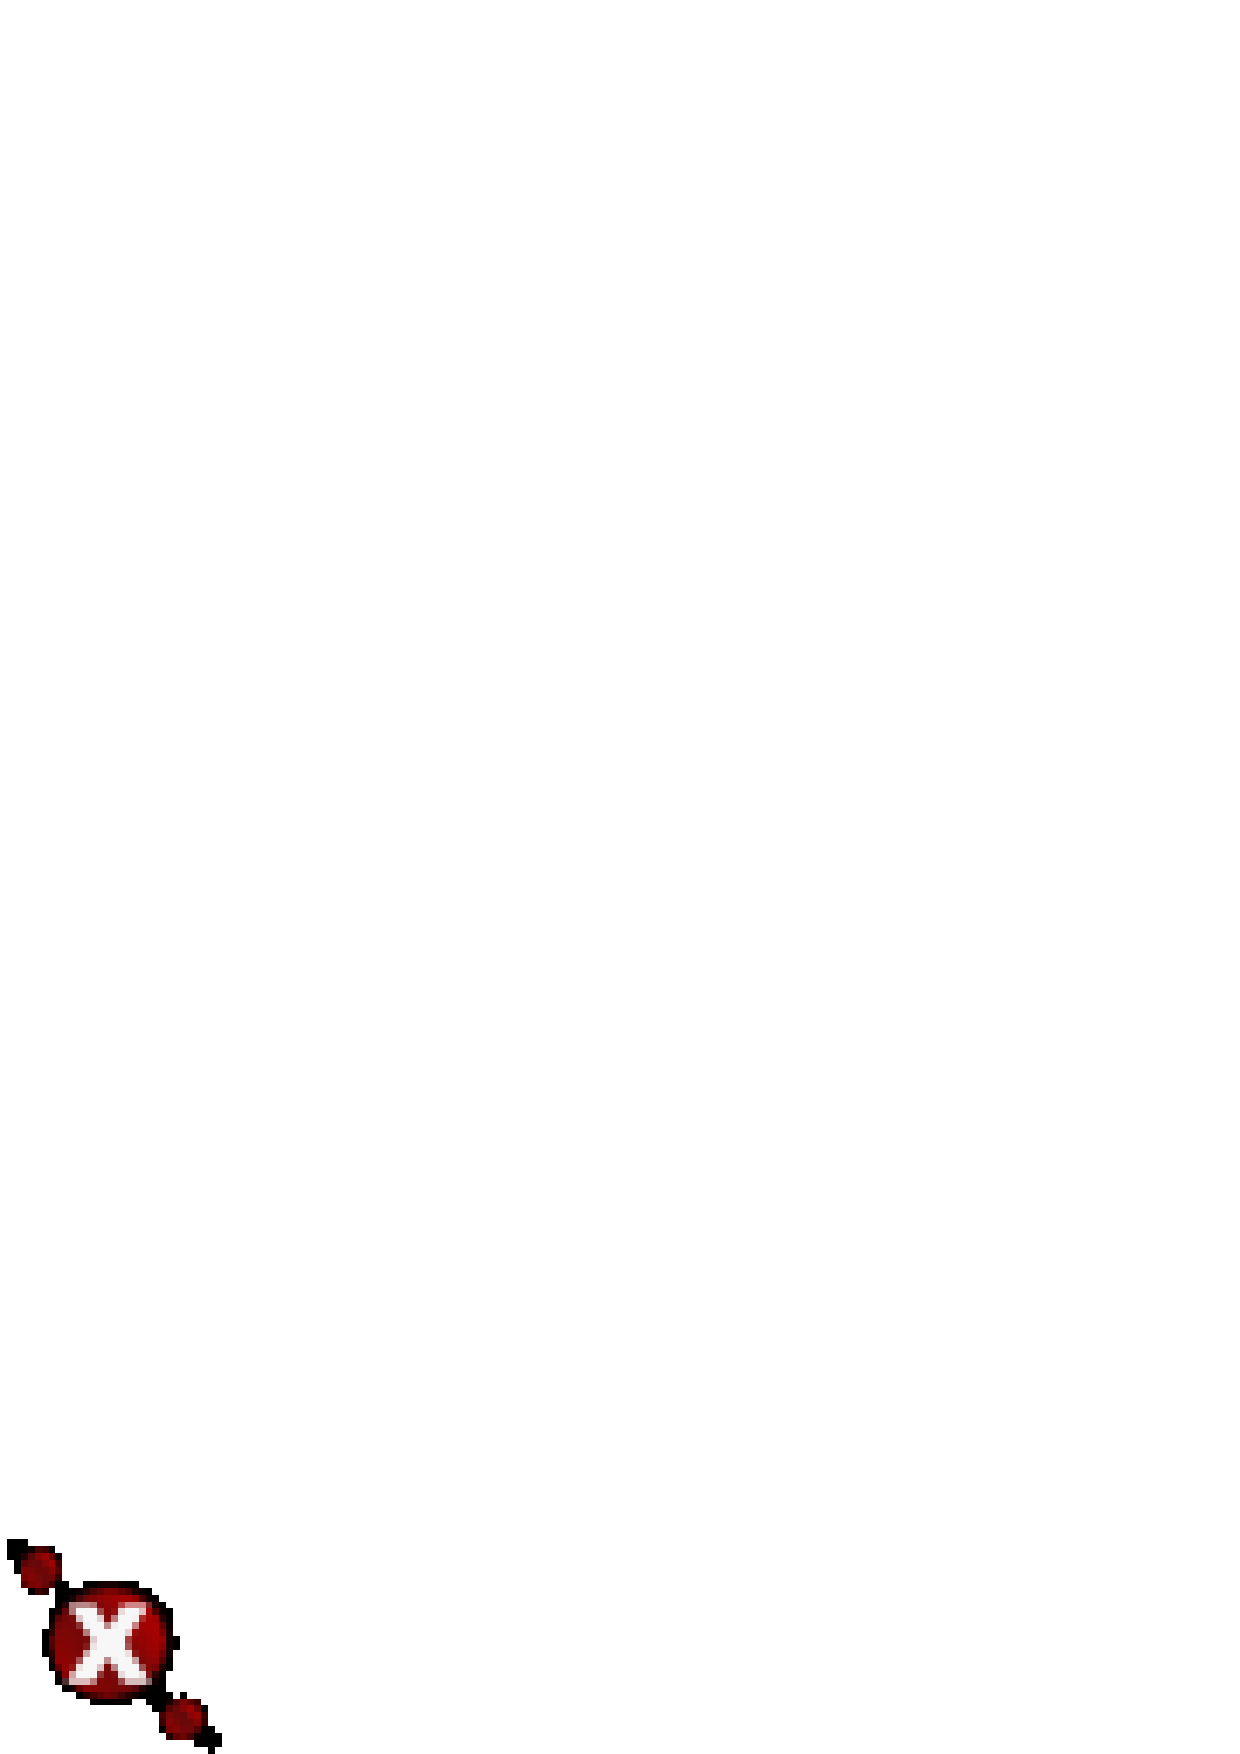
\includegraphics[width=0.7cm]{grass_delete_vertex} & Elimina vertice &
Cancella vertici da linee e contorni esistenti (confermare l'eliminazione del
vertice selezionato cliccando una seconda volta)\\
\hline 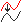
\includegraphics[width=0.7cm]{grass_move_line} & Sposta elemento &
Sposta il contorno, la linea, il punto o il centroide selezionato in una nuova
posizione\\
\hline 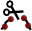
\includegraphics[width=0.7cm]{grass_split_line} & Dividi linea & Divide
una linea o un contorno in due parti nel punto selezionato (confermare
cliccando una seconda volta)\\
\hline 
\includegraphics[width=0.7cm]{grass_delete_line} & Elimina elemento &
Elimina un contorno, una linea, un punto o un centroide esistente (confermare
cliccando una seconda volta)\\
\hline 
\includegraphics[width=0.7cm]{grass_edit_attributes} & Modifica
attributi & Modifica gli attributi dell'elemento selezionato (si noti che ad un
elemento possono essere associati più attributi, si veda sopra)\\
\hline 
\includegraphics[width=0.7cm]{grass_close_edit} & Chiudi & Chiude la
sessione e salva lo stato attuale (ricostruisce la topologia)\\
\hline
\end{tabular}
\end{table}

\minisec{Scheda Categoria}\index{GRASS!impostazioni categoria}

La scheda \tab{Categoria} consente di definire il modo in cui i valori
della categoria verranno assegnati al nuovo elemento geometrico.

\begin{figure}[h]
 \centering
  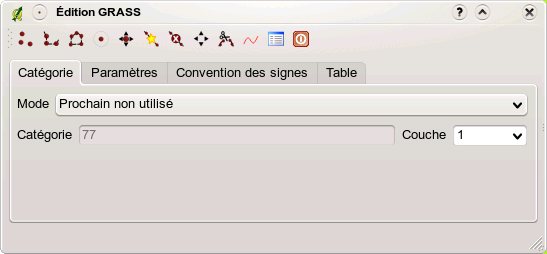
\includegraphics[clip=true,width=8cm]{grass_digitizing_category}
  \caption{Scheda Categoria \nixcaption}\label{fig:grass_digitizing_category}
 \end{figure}

\begin{itemize}[label=--]
\item \textbf{Modalità}: modalità con la quale viene assegnata la categoria
(colonna cat della tabella) alle geometrie digitalizzate.
\begin{itemize}
\item Prossimo non in uso - applica il primo valore non utilizzato in ordine
numerico crescente.
\item Inserimento manuale - definizione manuale della categoria da assegnare
all'elemento.
\item Nessuna categoria - non assegna alcun valore all'elemento. Questa
modalità è in genere usata ad esempio per i contorni dei poligoni ai quali la
categoria viene collegata tramite il centroide.
\end{itemize}
\item \textbf{Categoria} - Il numero (ID) inserito o visualizzato viene
associato ad ogni elemento digitalizzato. Viene usato per collegare ogni
elemento geometrico ai relativi attributi.
\item \textbf{Layer} - Ogni elemento geometrico può essere collegato
con molteplici tabelle attributo usando diversi livelli (``layer'') secondo il
modello GRASS: il numero del layer predefinito è 1. 
\end{itemize}

\begin{Tip}\caption{\textsc{Creare un livello GRASS aggiuntivo con QGIS}}
Se si vogliono aggiungere ulteriori livelli al set di dati, inserire
semplicemente un numero nel campo ``Layer'' e dare invio. Nella scheda
Tabella sarà a questo punto possibile creare il nuovo schema degli attributi
da associare a questo livello.
\end{Tip}

\minisec{Scheda Preferenze}\label{label_settingtab}\index{GRASS!tolleranza snap}

La scheda \tab{Preferenze} consente di impostare la tolleranza per
l'aggancio automatico tra elementi (snapping) in pixels dello schermo. La
soglia definisce a quale distanza massima nuovi punti o linee sono agganciati
ad altri nodi esistenti. Ciò aiuta ad evitare interruzioni o incroci tra
contorni. Il valore preimpostato è 10 pixels.

\begin{figure}[h]
 \centering
 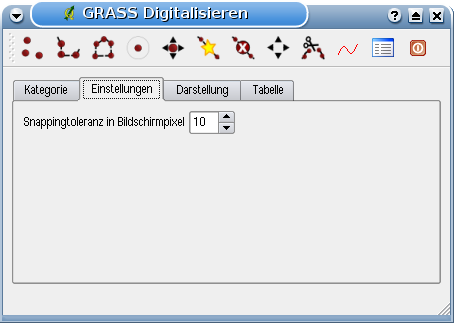
\includegraphics[clip=true,width=8cm]{grass_digitizing_settings}
 \caption{Scheda Preferenze \nixcaption}\label{fig:grass_digitizing_settings}
\end{figure}

\minisec{Scheda Simbologia}\index{GRASS!impostazioni simbologia}

La scheda \tab{Simbologia} consente di visualizzare e impostare la
simbologia e i colori dei vari tipi geometrici nei vari stati topologici (ad
es. contorni aperti/chiusi).

\begin{figure}[h]
 \centering
 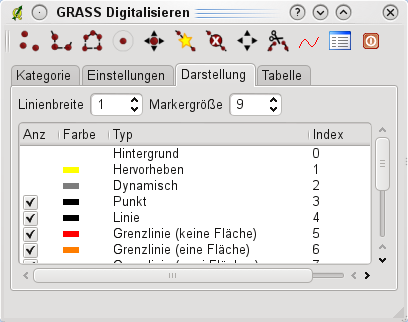
\includegraphics[clip=true,width=8cm]{grass_digitizing_symbology}
 \caption{Scheda Simbologia \nixcaption}\label{fig:grass_digitizing_symbology}
\end{figure}

\minisec{Scheda Tabella} \index{GRASS!modifica tabella}

La scheda \tab{Tabella} fornisce informazioni sulla struttura della tabella
per un determinato livello. È possibile aggiungere nuove
colonne ad una tabella attributi esistente o creare un nuovo schema tabella
per un nuovo layer vettoriale GRASS o per un nuovo livello (Sezione \ref{sec:creating_new_grass_vectors}).

\begin{figure}[h]
 \centering
 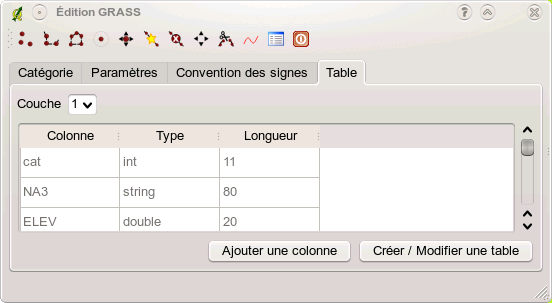
\includegraphics[clip=true,width=10cm]{grass_digitizing_table}
 \caption{Scheda Tabella \nixcaption}\label{fig:grass_digitizing_table}
 \end{figure}

\begin{Tip}\caption{\textsc{Permessi di modifica in GRASS}}\index{GRASS!modifica permessi}
È necessario essere il proprietario del \filename{MAPSET} GRASS che
si vuole editare. Non è possibile modificare dati in un {MAPSET} del quale non
si è proprietari, anche se si possiedono su di esso permessi in scrittura.
\end{Tip} 

\section{Lo strumento Regione di GRASS}\label{sec:grass_region}\index{GRASS!region}

L'impostazione di una regione (ovvero di una porzione di spazio geografico
nella quale operare) è molto importante in GRASS, specialmente quando si lavora con dati
raster. L'analisi vettoriale non è limitata
all'impostazione della regione ma interessa tutta l'estensione del
layer. Tutti i raster di nuova creazione avranno l'estensione e la risoluzione
spaziale della regione GRASS definita, indipendentemente dalla loro estensione
e risoluzione originale. L'impostazione corrente della regione GRASS è salvata
nel file \filename{\$LOCATION/\$MAPSET/WIND} che ne definisce i limiti nord, sud
est e ovest, il numero di righe e colonne e la risoluzione spaziale in senso
orizzontale e verticale.

È possibile abilitare/disabilitare la visualizzazione della regione di GRASS
nella vista mappa in QGIS usando il pulsante \toolbtntwo{grass_region}{Visualizza la regione di GRASS attuale}. \index{GRASS!region!visualizza}

Con lo strumento \toolbtntwo{grass_region_edit}{Modifica la regione di GRASS attuale}
è possibile aprire una finestra di dialogo per cambiare le impostazioni
correnti della regione e la simbologia con la quale il rettangolo che la
rappresenta viene visualizzato nella vista mappa di QGIS. Inserire i nuovi
limiti della regione e la risoluzione e cliccare su \button{OK}. Lo strumento
consente anche di selezionare l'estensione della regione interattivamente con
il mouse nella vista mappa di QGIS. Cliccando con il tasto sinistro del
mouse nella vista mappa si imposta il primo angolo del rettangolo che definirà
la regione e cliccando in un altro punto lo si chiuderà: cliccare su
\button{OK} per confermare.\index{GRASS!region!modifica}
Il modulo GRASS \filename{g.region} mette a disposizione molti più parametri
per definire l'estensione della regione e la risoluzione con la quale si vuole
condurre l'analisi raster. Si possono usare questi parametri tramite lo
strumento GRASS appropriato (Sezione \ref{subsec:grass_toolbox}).

\section{Gli strumenti GRASS}\label{subsec:grass_toolbox}\index{GRASS!strumenti}

Cliccando su \toolbtntwo{grass_tools}{Apri strumenti GRASS} si ha accesso
alle funzionalità dei moduli GRASS con i quali lavorare nella
\filename{LOCATION} e nel \filename{MAPSET} impostati. Per usare gli strumenti
di GRASS è necessario aprire una \filename{LOCATION} e un \filename{MAPSET}
sui quali si abbiano permessi di scrittura (in genere concessi se si è
l'utente che ha creato il \filename{MAPSET}). Ciò è necessario in quanto i
nuovi layer raster o vettoriali creati durante l'analisi devono poter essere
scritti nella \filename{LOCATION} e nel \filename{MAPSET} selezionati.

\subsection{Elenco dei moduli GRASS con interfaccia grafica}\index{GRASS!toolbox!moduli grafic}

È possibile trovare la lista completa dei moduli GRASS accessibili tramite l'interfaccia grafica di QGIS 
nel wiki di GRASS: \url{http://grass.osgeo.org/wiki/GRASS-QGIS_relevant_module_list}

\subsection{Lavorare con i moduli GRASS}\label{subsec:grass_modules}\index{GRASS!strumenti}

\begin{figure}[ht]
\centering
   \subfloat[Albero modulil] {\label{subfig:grass_module_tree}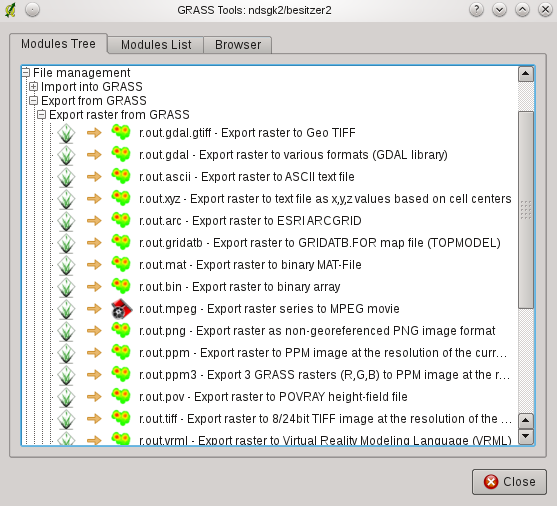
\includegraphics[clip=true, width=0.4\textwidth]{grass_toolbox_moduletree}}
   \hspace{0.5cm}
   \subfloat[Lista moduli] {\label{subfig:grass_module_list}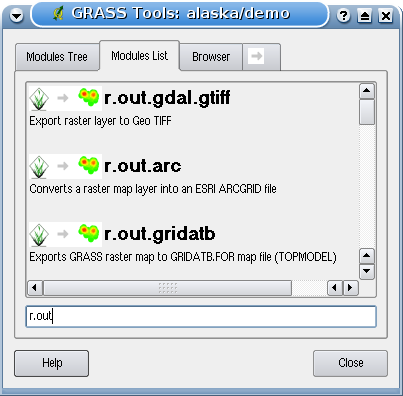
\includegraphics[clip=true, width=0.4\textwidth]{grass_toolbox_modulelist}}
\caption{La finestra di dialogo degli strumenti GRASS \nixcaption}\label{fig:grass_modules}
\end{figure}

La shell di GRASS fornisce accesso a praticamente tutti gli oltre 300 moduli GRASS 
in modalità riga di comando. Per offrire un ambiente di
lavoro maggiormente user-friendly, circa 200 di questi moduli e loro relative
funzionalità sono presentati in finestre di dialogo. Questi moduli sono
raggruppati in blocchi tematici: è disponibile una funzione di ricerca. 

È possibile personalizzare il contenuto della finestra di dialogo degli strumenti GRASS: la procedura 
è descritta nella Sezione \ref{sec:toolbox-customizing}.

Come mostrato in Figura \ref{fig:grass_modules}, è possibile ricercare il modulo
GRASS desiderato per aree tematiche nella scheda \tab{Albero
moduli} o nella scheda \tab{Lista moduli} che permette la ricerca per parola chiave. 

Cliccando sull'icona di un modulo grafico verrà aggiunta una nuova scheda
alla finestra di dialogo degli strumenti. In questa scheda si avranno tre ulteriori
sottoschede denominate \tab{Opzioni}, \tab{Output} e \tab{Manuale}. Un
esempio è mostrato in Figura \ref{fig:grass_module_dialog} per il modulo
\filename{v.buffer}.

\begin{figure}[h]
\centering
   \subfloat[Scheda Opzioni] {\label{subfig:grass_module_option}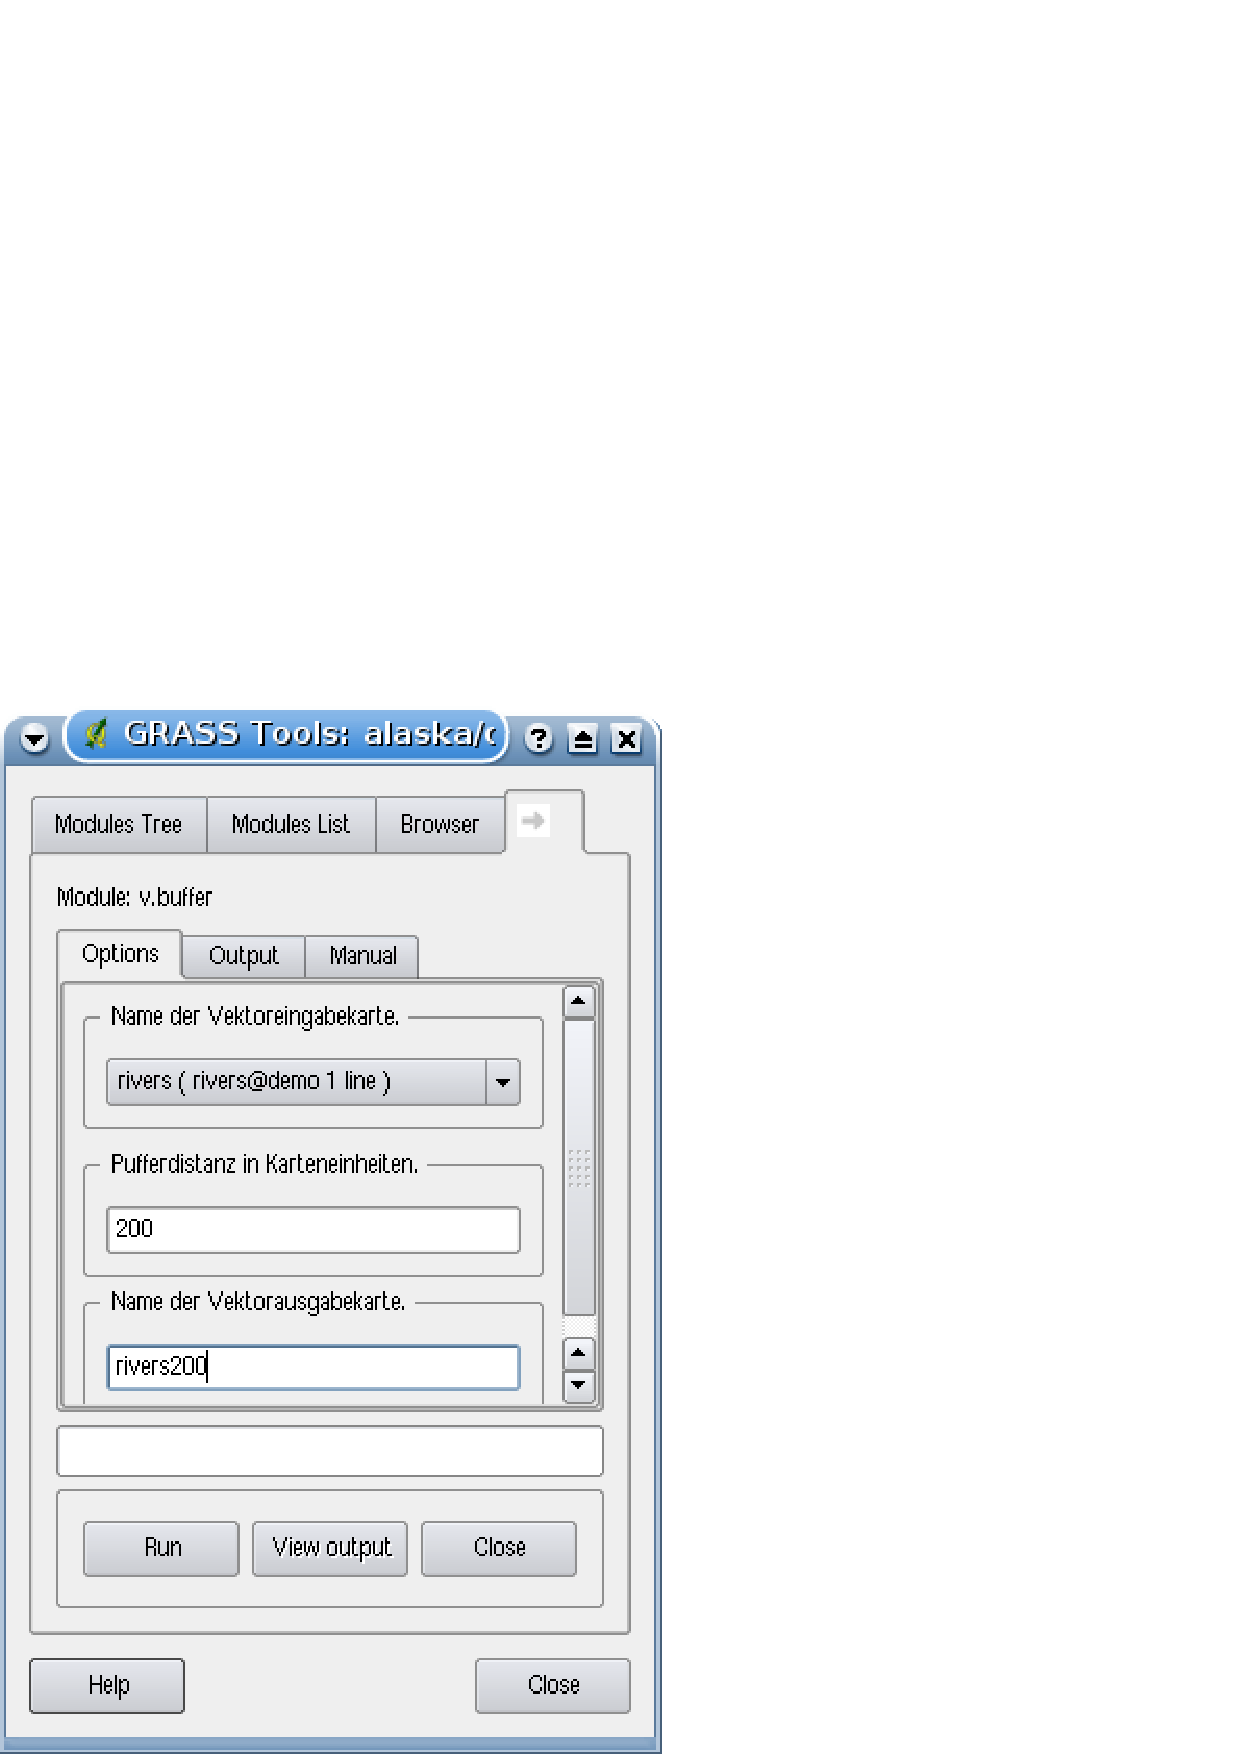
\includegraphics[clip=true, width=0.3\textwidth]{grass_module_option}}
   \hspace{1cm}
   \subfloat[Scheda Output] {\label{subfig:grass_module_output}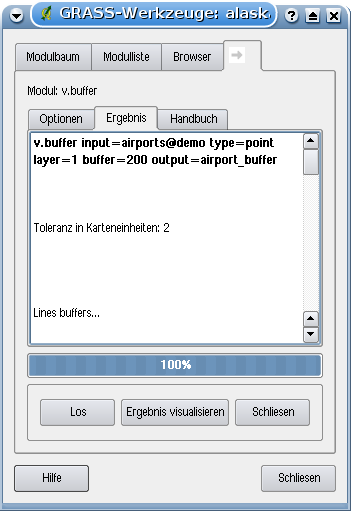
\includegraphics[clip=true, width=0.3\textwidth]{grass_module_output}}
   \hspace{1cm}
   \subfloat[Scheda Manuale] {\label{subfig:grass_module_manual}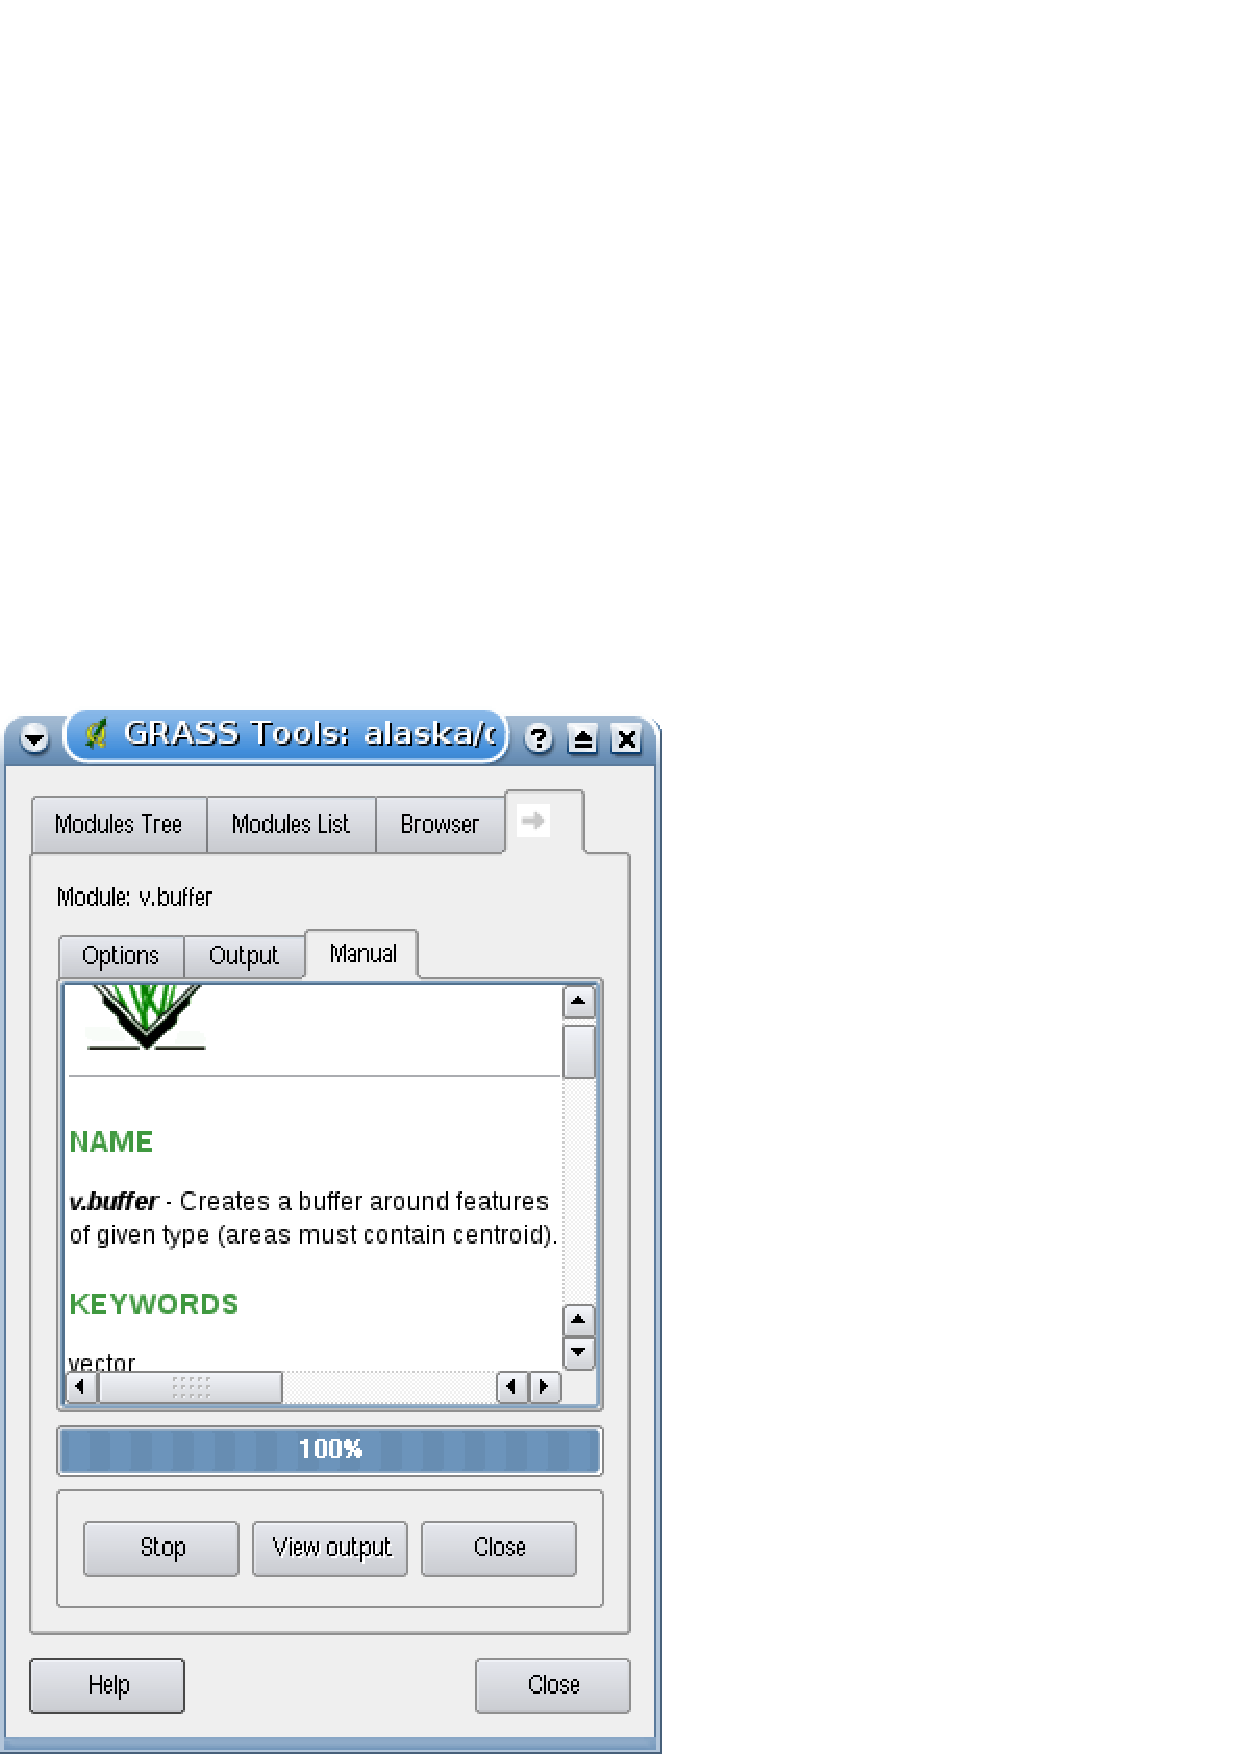
\includegraphics[clip=true, width=0.3\textwidth]{grass_module_manual}}
\caption{Finestre di dialogo di un modulo GRASS \nixcaption}\label{fig:grass_module_dialog}
\end{figure}
\FloatBarrier

\minisec{Opzioni}

La scheda \tab{Opzioni} fornisce una finestra semplificata nel quale di
solito è possibile selezionare un layer raster o vettoriale ed inserire
ulteriori opzioni specifiche per l'esecuzione del modulo. Per mantenere la
leggibilità della finestra non sempre sono presenti tutte le opzioni: qualora si
volessero usare ulteriori parametri per il modulo è necessario avviare la
shell di GRASS ed eseguire il modulo dalla riga di comando.

Una nuova caratteristica di QGIS \CURRENT è il supporto per un pulsante
\button{Mostra le opzioni avanzate >>} nella scheda \tab{Opzioni} della 
finestra di dialogo semplificata di un modulo. Al momento tale funzionalità è 
disponibile per pochi moduli, ma probabilmente sarà estesa ad altri 
moduli nelle prossime versioni di QGIS. Ciò permetterà di sfruttare appieno le potenzialità 
dei moduli di GRASS senza dover usare la shell.

\minisec{Output}

La scheda \tab{Output} fornisce informazioni sull'avanzamento delle
operazioni eseguite dal modulo. Quando si clicca sul pulsante \button{Esegui},
viene portata in primo piano la scheda \tab{Output} nella quale vengono
visualizzate le informazioni sul processo in corso. Se l'operazione va a buon
fine, si vedrà il messaggio \usertext{Operazione conclusa con successo}.

\minisec{Manuale}

La scheda \tab{Manuale} mostra la pagina di aiuto in formato HTML del modulo
GRASS scelto: permette di verificare la disponibilità di ulteriori
parametri o ottenere una conoscenza più approfondita delle operazioni che il
modulo può eseguire. Alla fine di ogni pagina di manuale vi sono ulteriori
collegamenti al \filename{Main Help index}, al \filename{Thematic index} o al
\filename{Full index}. Questi link forniscono le stesse informazioni che si
avrebbero usando il modulo \filename{g.manual}.

\begin{Tip}\caption{\textsc{Mostrare i risultati immediatamente}}\index{GRASS!visualizza risultato}
Se si desidera visualizzare il risultato di un'analisi immediatamente
nella vista mappa, è possibile cliccare sul pulsante "Visualizza Output" nella
porzione inferiore della scheda.
\end{Tip} 

\subsection{Esempi di utilizzo di moduli GRASS}\index{GRASS!strumenti}

Gli esempi che seguono mostrano le potenzialità di alcuni moduli GRASS. 

\minisec{Creare curve di livello} 

Come primo esempio, deriviamo le curve di livello a partire da un modello 
digitale di elevazione (DEM): si assume che la \filename{LOCATION} Alaska 
sia impostata come descritto nella Sezione \ref{sec:import_loc_data}. 

\begin{itemize}[label=--]
\item Aprire la 'location' Alaska cliccando su \toolbtntwo{grass_open_mapset}{Apri mapset}.
\item Caricare il DEM \usertext{gtopo30} cliccando su 
\toolbtntwo{grass_add_raster}{Aggiungi raster GRASS} e selezionando \usertext{gtopo30} 
dal mapset demo.
\item Aprire gli strumenti GRASS con \toolbtntwo{grass_tools}{Apri strumenti GRASS}. 
\item Nell'albero dei moduli cliccare su Raster \arrow Gestione superficie \arrow Genera curve di livello vettoriali. 
\item Cliccando su \classname{r.contour} si aprirà la finestra di dialogo dello strumento
come spiegato in \ref{subsec:grass_modules}. Il raster \usertext{gtopo30} dovrebbe 
apparire in \inputtext{Nome della mappa raster in input}{gtopo30}. 
\item Inserire in \inputtext{Incremento fra le isoipse}{100} il valore 100 
(per creare curve di livello ad intervalli di 100 metri).
\item Inserire in \inputtext{Nome del vettoriale in output}{ctour\_100}
\usertext{ctour\_100}. 
\item Cliccare su \button{Esegui} ed attendere fino alla comparsa del messaggio 
\usertext{Operazione conclusa con successo}: quindi cliccare su \button{Visualizza risultato} 
e su \button{Chiudi}. 
\end{itemize}

\begin{figure}[ht]
\centering
   \subfloat[Opzioni di r.contour] {\label{subfig:grass_toolbox_rcontour}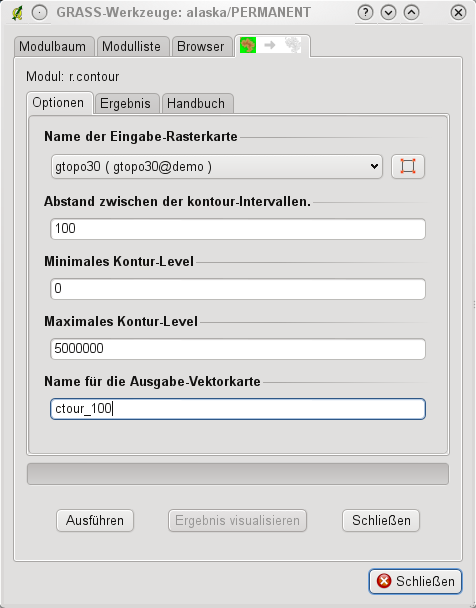
\includegraphics[clip=true, width=0.4\textwidth]{grass_toolbox_rcontour}}
    \hspace{0.5cm}
   \subfloat[Output di r.contour] {\label{subfig:grass_toolbox_rcontour2}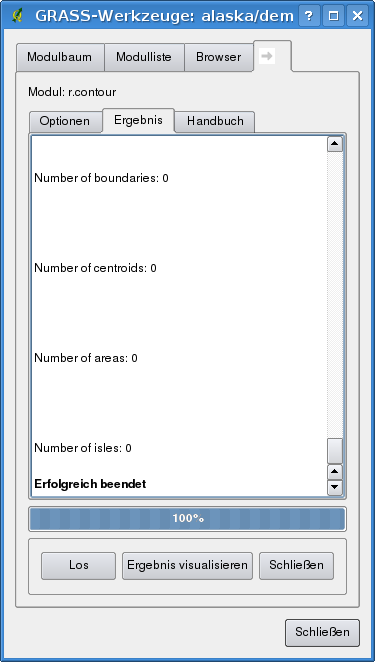
\includegraphics[clip=true, width=0.4\textwidth]{grass_toolbox_rcontour2}}
   \caption{\grass Modulo GRASS r.contour \nixcaption}\label{fig:grass_toolbox_rcontour}
\end{figure}

Una volta terminata l'operazione è possibile modificare le proprietà del nuovo layer 
vettoriale come descritto in \ref{sec:vectorprops}.

Ingrandendo una porzione della mappa in un'area più montagnosa si potrà 
notare come le curve di livello appaiano spigolose. In GRASS è disponibile 
il modulo \classname{v.generalize} per alterare leggermente un vettore senza 
modificarne la forma generale: il modulo utilizza diversi algoritmi, ognuno per 
uno scopo specifico. Alcuni algoritmi (es. Douglas Peuker e Vertex reduction) 
semplificano una linea rimuovendo alcuni vertici: il risultato sarà più veloce 
da caricare. Tale tipo di algoritmo è ad esempio molto utile nel caso in cui si 
abbia una mappa vettoriale molto dettagliata, ma si sta lavorando ad una scala 
molto piccola per cui tanto dettaglio non è necessario.

\begin{Tip}\caption{\textsc{Semplifica geometrie}}\index{GRASS!visualizza risultato}
Si noti che lo strumento \toolbtntwo{simplify_ft}{Semplifica geometrie} di fTools 
opera allo stesso modo dell'algoritmo Douglas-Peuker di \classname{v.generalize}. 
\end{Tip}  

Ad ogni modo, lo scopo dell'esempio è diverso: le curve di livello create con r.contour 
hanno angoli molto acuti che devono essere smussati. Tra gli algoritmi di 
\classname{v.generalize} Chaikens (o anche Hermite splines) fa al caso nostro. 
Si noti che l'algoritmo potrebbe \textbf{aggiungere} dei vertici, rendendo il caricamento 
della mappa ancora più lento.

\begin{itemize}[label=--]
\item Aprire gli strumenti di GRASS e lanciare il modulo Vettore \arrow
Elabora mappa \arrow Generalizzazione \arrow \classname{v.generalize}.
\item Controllare che \usertext{ctour\_100} appaia come 
\inputtext{Nome della mappa vettoriale in input}{ctour\_100}. 
\item Scegliere Chaiken's come algoritmo di generalizzazione ed inserire il
\inputtext{Nome del vettoriale in output}{ctour\_100\_smooth}
\item Cliccare su \button{Esegui} ed attendere fino alla comparsa del messaggio 
\usertext{Operazione conclusa con successo}: quindi cliccare su \button{Visualizza risultato} 
e su \button{Chiudi}. 
\item È possibile modificare il colore del layer vettoriale in modo da renderlo ben 
visibile sul raster si sfondo. Si potrà notare come le curve di livello ora appaiano
meno spigolose.
\end{itemize}

\begin{figure}[h]
 \centering
 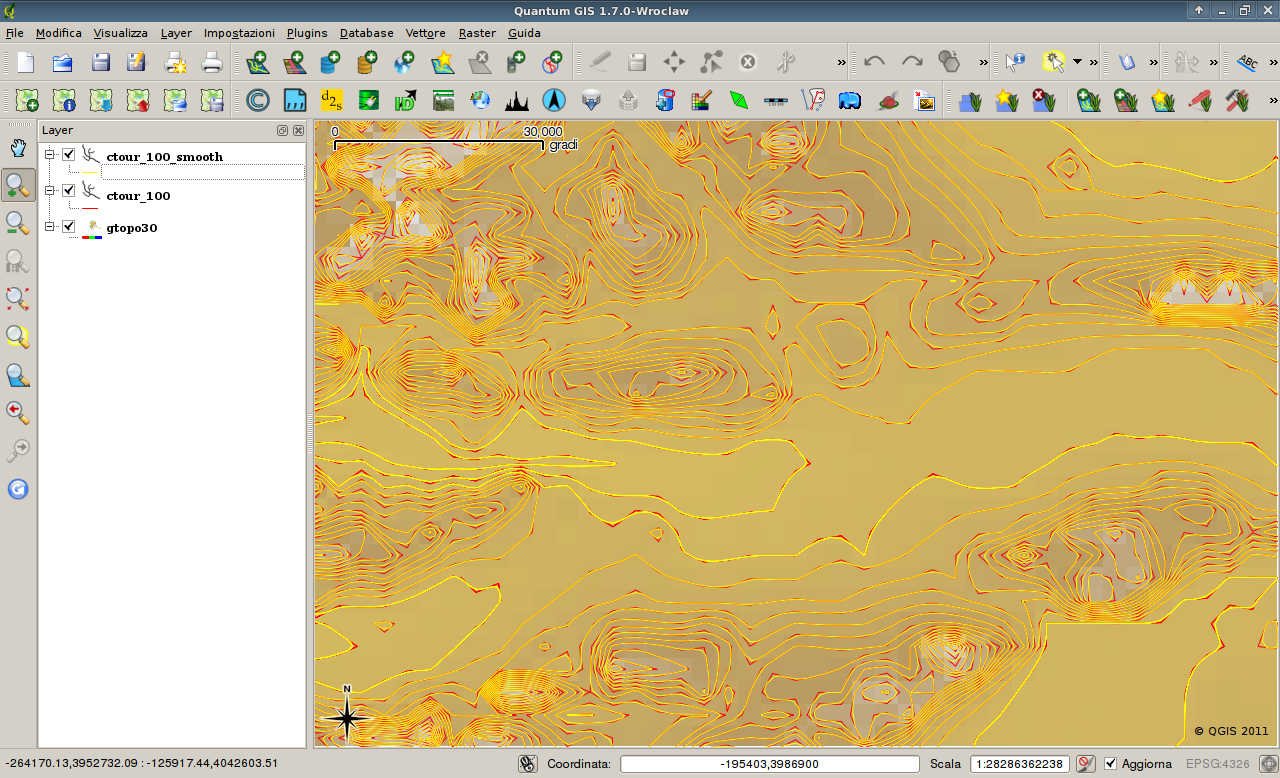
\includegraphics[clip=true, width=14cm]{grass_toolbox_vgeneralize}
 \caption{Module GRASS v.generalize \nixcaption}\label{fig:grass_toolbox_vgeneralize}
\end{figure}

\begin{Tip}\caption{\textsc{Altri usi di r.contour}}\index{GRASS!strumenti}
La procedura appena descritta può essere usata in situazioni equivalenti.
Se si ha un raster delle precipitazioni, ad esempio, si può usare r.contour per 
derivare le isoiete (curve a precipitazione costante).
\end{Tip}  

\minisec{Creare un rilievo ombreggiato con effetto 3D}

Ci sono diversi modi per visualizzare dati di elevazione e dare un effetto 3D alla vista.
L'uso delle curve di livello è uno dei metodi più utilizzato, sopratutto nella 
produzione di mappe topografiche. 
Un altro modo consiste nell'utilizzare l'ombreggiatura. L'ombra viene derivata da un 
DEM, calcolando prima pendenze ed orientamento, poi simulando la posizione del sole 
nel cielo per assegnare un valore di riflettanza per ogni cella del raster: in tal modo 
le pendenze in ombra saranno più scure di quelle esposte al sole.

\begin{itemize}[label=--]
\item Caricare il raster \usertext{gtopo30}, aprire gli strumenti di GRASS e lanciare
il modulo Raster \arrow Analisi spaziali \arrow Analisi geomorfologica \arrow \classname{r.shaded.relief}.
\item Impostare l'\inputtext{azimuth}{270} a 315 ed inserire \usertext{gtopo30\_shade} 
in \inputtext{Output shaded relief map name}{gtopo30\_shade} (Il nome del raster in output).
\item Cliccare su \button{Esegui} ed attendere fino alla comparsa del messaggio 
\usertext{Operazione conclusa con successo}: quindi cliccare su \button{Visualizza risultato} 
e su \button{Chiudi}. 
\item Il nuovo raster verrà visualizzato in scala di grigi: per vedere contemporaneamente 
l'ombreggiatura ed i colori di \usertext{gtopo30}, portare \usertext{gtopo30\_shade} 
sotto \usertext{gtopo30} nella legenda, quindi aprire le \dropmenuopt{Proprietà} di 
\usertext{gtopo30}, andare nella scheda \tab{Trasparenza} ed impostare il livello di 
trasparenza al 25\%. 
\end{itemize}

\minisec{Usare la shell di GRASS}
 
Il plugin GRASS è orientato principalmente agli utenti che non conoscono 
GRASS ed i suoi moduli, con relative opzione, per cui molti moduli non 
mostrano tutte le possibili opzione ed altri non sono affatto presenti.

La shell di GRASS consente di accedere ai moduli che non appaiono 
nell'interfaccia grafica ed alle opzioni aggiuntive di quelli che invece ci sono.
Il seguente esempio mostra l'uso di un'opzione del modulo \classname{r.shaded.relief}.

\begin{figure}[ht]
 \centering
 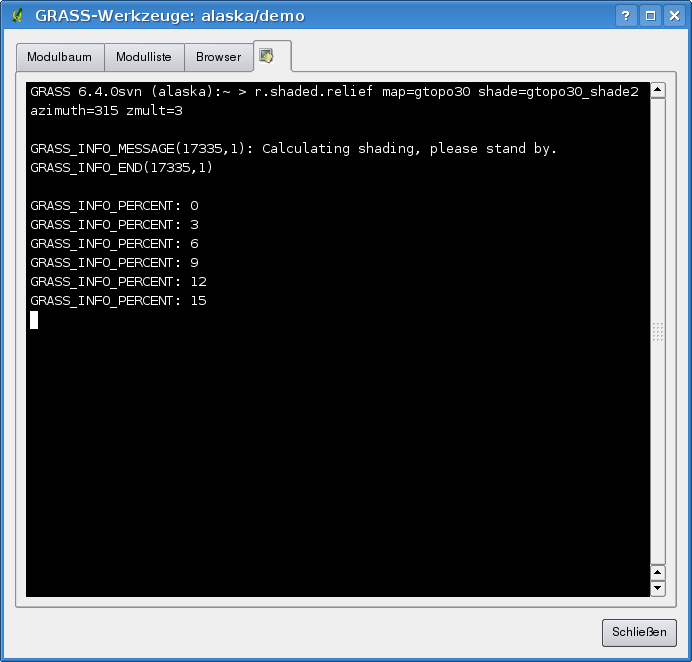
\includegraphics[clip=true, width=12cm]{grass_toolbox_shell}
 \caption{La shell di GRASS ed il modulo r.shaded.relief \nixcaption}\label{fig:grass_toolbox_shell}
\end{figure}

Il modulo \classname{r.shaded.relief} può utilizzare il parametro \usertext{zmult}
che amplifica il valore dell'elevazione in modo tale che l'effetto di ombreggiatura 
sia più pronunciato.

\begin{itemize}[label=--]
\item Caricare \usertext{gtopo30} ed aprire la shell di GRASS. Nella shell scrivere 
il comando:\linebreak
\usertext{r.shaded.relief map=gtopo30 shade=gtopo30\_shade2 azimuth=315
zmult=3} \linebreak e premere \keystroke{Invio}.
\end{itemize}

\begin{itemize}[label=--]
\item Quando il comando ha terminato, spostarsi nella scheda \tab{Browser} della 
finestra di dialogo degli strumenti GRASS e fare doppio click sul nuovo raster 
\usertext{gtopo30\_shade2} per visualizzarlo in QGIS. 
\item Impostare le proprietà del raster così come descritto in precedenza.
\end{itemize}

\begin{figure}[ht]
 \centering
 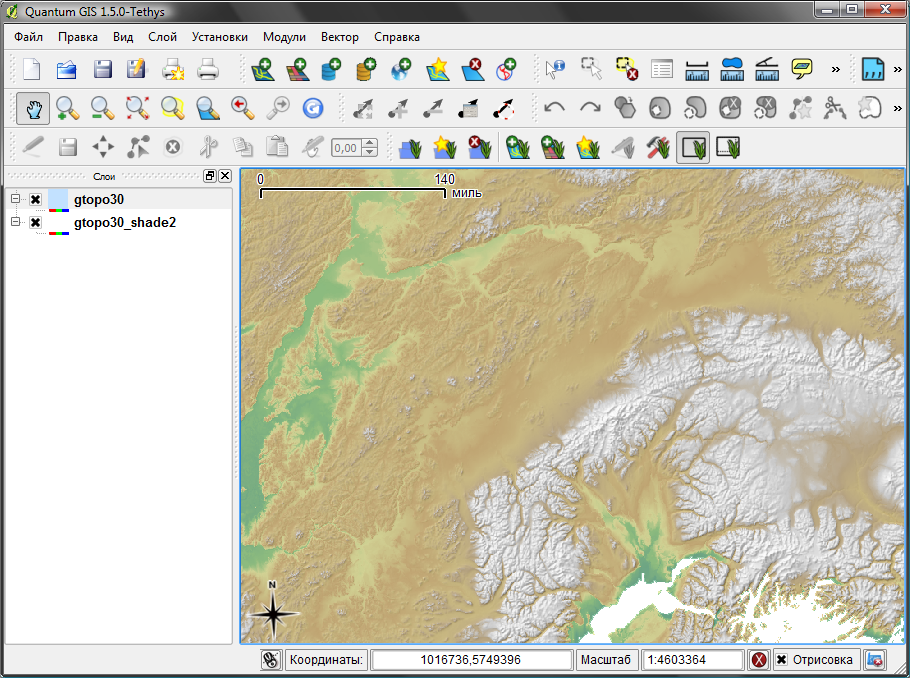
\includegraphics[clip=true, width=12cm]{grass_toolbox_shadedrelief}
 \caption{Rilievo ombreggiato creato con il modulo GRASS r.shaded.relief \nixcaption}\label{fig:grass_toolbox_shadedrelief}
\end{figure}

\minisec{Statistiche raster in una mappa vettoriale}

Il prossimo esempio tratta di un modulo GRASS che può aggregare 
dati raster ed aggiungere colonne di statistiche per ogni poligono di una 
mappa vettoriale.

\begin{itemize}[label=--]
\item Importare in GRASS lo shapefile \filename{trees} nella cartella \usertext{shapefiles} 
(Sezione \ref{sec:import_loc_data}).
\item Prima di proseguire bisogna aggiungere i centroidi ai poligoni 
per farne delle aree vettoriali secondo il modello dati di GRASS. 
\item Aprire gli strumenti di GRASS e lanciare il modulo 
Vettore \arrow Elabora mappa \arrow Gestisci elementi \arrow \classname{v.centroids}. 
\item Inserire \inputtext{Name of output vector map}{\usertext{trees\_areas}}
e lanciare il modulo. 
\item Caricare \usertext{trees\_areas} e visualizzare le categorie - deciduous, evergreen, mixed trees - 
con colori differenti. Aprire le \dropmenuopt{Proprietà} del layer, 
andare nella scheda \tab{Stile}, scegliere il visualizzatore Categorizzato
ed impostare la colonna \inputtext{Colonna}{VEGDESC} (Sezione \ref{sec:symbology}).
\item Aprire il modulo GRASS Vettore \arrow Aggiornamento di un vettore da altre mappe \arrow 
\classname{v.rast.stats}. Inserire \inputtext{Name of
raster map to calculate statistics from}{\usertext{gtopo30}} e \inputtext{Name of vector
polygon map}{\usertext{trees\_areas}}. 
\item Inserire \inputtext{Column prefix for new attribute columns}{\usertext{elev}} e
cliccare su \button{Esegui}: l'operazione potrebbe durare molto tempo. 
\item Aprire la tabella degli attributi di \usertext{trees\_areas} e verificare come 
siano state aggiunte diverse nuove colonne, come ad esempio \usertext{elev\_min},
\usertext{elev\_max}, \usertext{elev\_mean}, per ogni tipo di poligono.
\end{itemize}

\subsection{Lavorare con il browser delle LOCATION GRASS} \index{GRASS!strumenti!browser}

Un'altra utile funzione tra quelle presenti negli strumenti GRASS è il browser
delle \filename{LOCATION}. In Figura~\ref{fig:grass_mapset_browser} è
possibile vedere un esempio che mostra la \filename{LOCATION} impostata 
e i relativi \filename{MAPSET}.

Nella parte sinistra della finestra del browser si può navigare attraverso
tutti i \filename{MAPSET} contenuti nella \filename{LOCATION} impostata. La
porzione di destra mostra invece alcuni metadati del raster o del vettoriale
selezionato, come la risoluzione, l'estensione spaziale, la fonte del dato, il
percorso alla tabella attributi associata per i dati vettoriali e lo storico
comandi che ha generato quel dato.

\begin{figure}[h]
 \centering
 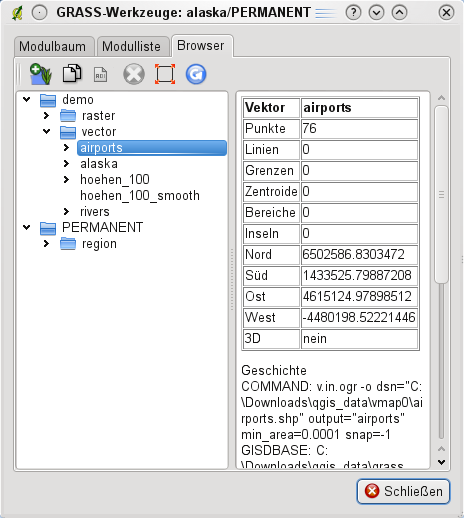
\includegraphics[clip=true,width=10cm]{grass_mapset_browser}
 \caption{Browser delle LOCATION GRASS \nixcaption}\label{fig:grass_mapset_browser}
\end{figure}

La barra degli strumenti nella scheda \tab{Browser} offre i seguenti
strumenti per la gestione della \filename{LOCATION} selezionata:

\begin{itemize}[label=--]
\item \toolboxtwo{grass_add_map}{Aggiungi la mappa selezionata all'area di
lavoro}
\item \toolboxtwo{grass_copy_map}{Copia la mappa selezionata}
\item \toolboxtwo{grass_rename_map}{Rinomina la mappa selezionata}
\item \toolboxtwo{grass_delete_map}{Elimina la mappa selezionata}
\item \toolboxtwo{grass_set_region}{Imposta la regione corrente con la mappa
selezionata}
\item \toolboxtwo{grass_refresh}{Aggiorna}
\end{itemize}

Gli strumenti \toolboxtwo{grass_rename_map}{Rinomina la mappa selezionata} e
\toolboxtwo{grass_delete_map}{Elimina la mappa selezionata} funzionano solo su
mappe contenute nel \filename{MAPSET} attivo. Tutti gli altri strumenti
funzionano anche con layer raster e vettoriali di altri \filename{MAPSET}.

\subsection{Personalizzare gli strumenti GRASS} \index{GRASS!strumenti!personalizzare}
\label{sec:toolbox-customizing}

Praticamente tutti i moduli GRASS possono essere aggiunti nella finestra di 
dialogo degli strumenti GRASS.
Per incorporare i file XML di configurazione dei moduli è fornita
un'interfaccia XML nella quale è possibile definire l'aspetto del modulo 
e i parametri da visualizzare nella finestra di dialogo degli strumenti.

Un esempio di file XML che genera il modulo \usertext{v.buffer} (v.buffer.qgm)
ha il seguente aspetto:

\begin{verbatim}
<?xml version="1.0" encoding="UTF-8"?>
<!DOCTYPE qgisgrassmodule SYSTEM "http://mrcc.com/qgisgrassmodule.dtd">

<qgisgrassmodule label="Vector buffer" module="v.buffer">
        <option key="input" typeoption="type" layeroption="layer" />
        <option key="buffer"/>
        <option key="output" />
</qgisgrassmodule>
\end{verbatim}

Il parser legge questa definizione e crea una nuova scheda nella finestra di 
dialogo degli strumenti GRASS quando si seleziona il modulo. 
Informazioni più dettagliate su come aggiungere moduli, cambiare i gruppi di moduli ecc. 
sono reperibile sul Wiki di QGIS all'indirizzo \\
\url{http://wiki.qgis.org/qgiswiki/Adding\_New\_Tools\_to\_the\_GRASS\_Toolbox}.

\FloatBarrier